\documentclass{mini}
\ProvidesPackage{result_figures}[2011/02/23 v1.0 My own macros]

% PACKAGES
%------------------------------------------------------------------------------%
\usepackage[utf8]{inputenc}
\usepackage{tikz}
\usepackage{pgfplots}
\usepackage{wrapfig}

\usepackage{csquotes}
\usepackage{amsmath}
\usepackage{epigraph}
\usepackage[linesnumbered,ruled]{algorithm2e}
\usepackage{adjustbox}

\DeclareMathOperator*{\argmin}{arg\,min} %argmin
\DeclareMathOperator*{\argmax}{arg\,max} %argmax

\usepackage{floatrow}
% Table float box with bottom caption, box width adjusted to content
\newfloatcommand{capbtabbox}{table}[][\FBwidth]
\usepackage{caption}
\usepackage{subcaption}
\captionsetup{compatibility=false}

%%%

\usepackage{array}
% For tabulars
\newcolumntype{P}[1]{>{\centering\arraybackslash}p{#1}}


\usepackage{pdfpages}
\usepackage{graphicx}
\usepackage{longtable}
%\usepackage[export]{adjustbox}
%\usepackage{tabu}
\usepackage{xcolor,colortbl}
\usepackage{caption}
\usepackage{subcaption}
\usepackage{float}
\usepackage{wrapfig}
\usepackage{amsfonts}

% LOAD CUSTOM COMMANDS FROM A FILE
%------------------------------------------------------------------------------
\usepackage{result_figures}


% TITLE
%------------------------------------------------------------------------------%
\title{Finite automata for pattern recognition}
\titleaux{Automaty skończone w problemie rozpoznawania wzorców}
\author{Jakub Ciecierski}
\coauthor{Bartlomiej Dybisz}
\supervisor{prof. nzw. dr hab. inż. Wladyslaw Homenda}
\type{bachelor}
\discipline{Computer Science}
\monthyear{february 2016}
\date{\today}
\album{243260}

%------------------------------------------------------------------------------%

\begin{document}

\maketitle

\tableofcontents



\chapter*{Work Devision}

{\bf Jakub Ciecierski}
\begin{itemize}
    \item Particle Swarm Optimization.
    \item Automaton implementation.
    \item Language Similarity.
    \item Language Transformation Analysis.
    \item Project structure and compilation.
\end{itemize}

{\bf Bartlomiej Dybisz}
\begin{itemize}
    \item Hill-Climber.
    \item Language implementation.
    \item Classifier Quality measurements.
    \item Language Transformation functionality.
    \item Graphical User Interface.
\end{itemize}


\abstract
Recognizing faces, discriminating between apple and oranges or understand spoken words are tasks, which are remarkably easy to processes for most of us, but happens to be astoundingly complex processes for machines. Following thesis introduces a novel approach for building classifier based on  Deterministic Finite Automaton. Such an automaton will be able to distinguish between input elements and classify them correctly. Authors compare two approaches based on widely known and used optimization algorithms: Particle Swarm Optimization and Hill Climbing. 

\bigskip
\textsc{keywords}: pattern recognition, classifier, classification, deterministic finite automaton, dfa, automata, equivalence classes, native elements, foreign elements, particle swarm optimization, hill climbing

\abstract
Wiele zadań zgoła prostych dla większości z nas - jak chociażby rozpoznawanie twarzy, czy odróżnienie piernika od wiatraka, okazuje się zdumiewająco trudne dla maszyn. Niniejsza praca bada budowę klasyfikatora opartego stricte na Deterministycznym Automacie Skończonym - podejście, które nie było wcześniej stosowane. Automat taki powinien poprawnie rozróżniać i klasyfikować elementy. W trakcie badań użyte zostały dwie metody heurystyczne: Particle Swarm Optimisation oraz Hill Climber.

\bigskip
\textsc{keywords}: rozpoznawanie wzorców, klasyfikator, klasyfikacja, deterministyczny automat skończony, das, automaty, klasy równoważności, elementy obce, elementy natywne, particle swarm optimization, hill climbing

\chapter*{Introduction}
%---------------------------------------------------------------
Although lately, we develop vast amount of techniques and algorithms to cope with pattern searching problem, it was implicitly used over centuries. For instance, the extensive astronomical observations of Tycho Brahe in the 16th century allowed Johannes Kepler to discover the empirical laws of
planetary motion, which in turn provided a springboard for the development of classical mechanics \cite{bishop_book}.

Automatic pattern recognition is usually considered as an engineering area which focusses on the development and evaluation of systems that imitate or assist humans in their ability of recognizing patterns \cite{duch_uuu}. Normally system, which recognizes patterns, consists of many intermediate elements, among which one can find a classifier. Following thesis introduces a novel approach for building classifier solely based on  Deterministic Finite Automaton (further referred as DFA). Such an automaton will be able to distinguish between input elements and classify them correctly. The research copes only with problem of classifier construction, hence it may be useful for various input data types like e.g. hand written letters or gesture patterns.

To systematize naming scheme and maintain coherent with subject's literature, we would like to briefly go through the common structures used in the following work. When one deals with different object to recognize, all of them belong to some specific class. For example letters can belong to classes such as: 'a', 'b', 'c' etc. We can easily revert previous sentence and say that classes has objects, which we will call elements. What is more, each of the elements is represented by a feature vector. Such a vector describe corresponding element in features space, hopefully allowing to discriminate it from the others. In addition, our work assumes that all feature vectors will be represented in form of the words over some predefined alphabet. Alphabet naturally consists of alphabet symbols, to which from now on we will refer as symbols. As one probably know set of words can be described as a language. In this way we can equate classes with languages.

Authors provide step-by-step explanation of each part along with mathematical background needed to understand theory behind the project. The study begins in chapter~\ref{chap:prelim} where preliminary mathematical knowledge is presented.
After chapter~\ref{chap:patt_rec} the reader should become familiar with the concept of pattern recognition and classification methods. Chapter~\ref{chap:lan_theory} provides detailed mathematical foundations behind automata and languages used in this study. It introduces the concept of transformation between classes and languages, as well as the idea of constructing a classifier based on an automaton.

In chapter~\ref{chap:pso}, the heuristic optimization method called Particle Swarm Optimization (PSO) is defined. This state of the art algorithm can be applied to a wide range of problems. The
general algorithm behind PSO is explained in details. Moreover, it provides a guide which helps the reader in applying PSO to solve any problem of choice. In contrast, a simpler search algorithm called Hill Climber is presented in chapter~\ref{chap:hill_climbing}. Similarly, it provides the reader with general knowledge of the algorithm and means of applying it to solve specific problems.

Chapter~\ref{chap:classifier} gathers all of the concepts defined thus far and provides a step-by-step explanation behind classifier construction which includes application of previously defined optimization algorithms. The final part of the thesis is devoted to experiments and results.  Chapter~\ref{chap:experiments} defines all of the conducted experiments and the results together with conclusions are presented in chapter~\ref{chap:results}.

The implementation details can be found in the appendix~\ref{chap:domain}. The structure of the project and dependencies of all of the modules are explained.


\chapter{Preliminaries}\label{chap:prelim}
%---------------------------------------------------------------------
Following chapter provides summary of mathematical background needed to proceed with the paper. We assume that reader is familiar with basic concepts of language theory such as: what is a language and what does it mean that it is regular. In addition, it is crucial for reader to understand the idea of equivalence relation and equivalence classes, because they comprise a very essence and motivation of this work. Finally, we are trying to (as quickly as possible) dive into theorems and definitions which are useful from the point of view of further application, rather than spending time on deriving knowledge from beginning.
%---------------------------------------------------------------------
%---------------------------------------------------------------------
\section{Myhill-Nerode}
\begin{definition} \label{def:myhill}
    Relation induced by language $L$ is a binary relation $R_{L}$ in the set of words over alphabet of $L$ such that:
    \[
    (\forall{u,v \in \Sigma^{*}})(u R_{L} v \equiv ((\forall z \in \Sigma^{*}) uz \in L \Leftrightarrow vz \in L))
    \]
\end{definition}
What is more, we know that $R_{L}$ is an equivalence relation, hence it divides $\Sigma^{*}$ into equivalence classes.

In the theory of formal languages, the $Myhill-Nerode$ theorem provides a necessary and sufficient condition for a language to be regular. The theorem is named for John Myhill and Anil Nerode, who proved it at the University of Chicago in 1958 (Nerode 1958) \cite{Myhill_Nerode}.

\begin{theorem}[Myhill-Nerode Theorem]\label{Theorem:Myhill_Nerode}
    The following conditions are equivalent:
    \begin{enumerate}
        \item a language $L$ is accepted by a deterministic finite automaton $M = (Q,\Sigma,\delta,q_0,F)$,
        \item a language $L$ is a union of some classes of a right invariant equivalence relation with finite index,
        \item the relation $R_{L}$ induced by a language $L$ has finite index.
    \end{enumerate}
\end{theorem}

%---------------------------------------------------------------------
%---------------------------------------------------------------------
\section{Hamming Distance} \label{sec:hamming}

\begin{definition}
Hamming distance $H_d$ between two string of the same length is the number of positions at which the corresponding symbols differ.
\end{definition}

\begin{example} 
Let $w = John$ and $v = Jhon$. Notice that the symbols at positions two and three differ. Thus the Hamming distance between these two strings is $H_d(w,v) = 2$.
\end{example}


%---------------------------------------------------------------------
%---------------------------------------------------------------------
\section{Deterministic Finite Automaton} \label{sec:autom}
%\begin{definition}
Deterministic Finite Automaton is a system of five fields:
\begin{center}
    $A = (Q, \Sigma, \delta, q_0, F)$
\end{center}

where \\
$Q$ - finite set of states. \\
$\Sigma$ - Finite input alphabet. \\
$\delta$ - transition function. $\delta: Q \times \Sigma \rightarrow Q$ \\
$q_0$ - the initial state. $q_0 \in Q$ \\
$F$ - Set of accepting states. $F \subseteq Q$ \\
%\end{definition}

Table~\ref{fig:ttable_std} shows an exmaple transition table for the standard transition $\delta: Q \times \Sigma \rightarrow Q$.

%%%
%
% Standard Transition function
%
%%%
\begin{figure}[H]
    \CenterFloatBoxes
    \begin{floatrow}
        
        \ttabbox
        {
            \centering
            \setlength{\tabcolsep}{15pt}
            \renewcommand{\arraystretch}{1.5}
            \begin{tabular}{|P{1.0cm} || P{0.6cm} | P{0.6cm} |}
                \hline
                $\delta$ & a & b \\
                \hline
                \hline
                $\rightarrow$$q^-$ 		& $q_0$ & $q_1$ \\
                \hline
                $q_0 $ 		& $q_R$ & $q_R$ \\
                \hline
                $q_1 $ 		& $q_1$ & $q_1$ \\
                \hline
                $q_R$  					& $q_R$ & $q_R$ \\
                \hline
            \end{tabular}
        }
        {\caption{Transition table for A with $\delta: Q \times \Sigma \rightarrow Q$. The initial state: $q^-$}\label{fig:ttable_std}}
        
        %\ffigbox
        %  {\includegraphics[width=0.35\textwidth]%{images/automaton_example.jpg}}
        %  {\caption{Example of Automaton %A}\label{fig:automaton_ex}}
        %\killfloatstyle
        
    \end{floatrow}
\end{figure}


The binary representation of automaton might perhaps provide more adequate solution for a computer. Thus a new transition function is defined, $\delta^{'}: Q \times \Sigma \times Q \rightarrow \{0,1\}$. It simply provides an answer whether there exists a transition between two states for a given symbol. For example, by looking at figure~\ref{fig:ttable_std} we can define value for $\delta^{'}(q^-,a,q_0) = 1$, since there exists a transition from $q^-$ to $q_0$ through symbol $a$. The entire automaton is presented in figure~\ref{fig:ttable_bin}.


%%%
%
% Binary transition function.
%
%%%
\begin{figure}[H]
    \begin{center}
        
        \setlength{\tabcolsep}{4pt}
        \renewcommand{\arraystretch}{1.4}
        
        \begin{subfigure}{.5\textwidth}
            
            \centering
            \begin{tabular}{|P{1.0cm} || P{0.8cm} | P{0.8cm} | P{0.8cm} | P{0.8cm}|}
                
                \hline
                a & $\rightarrow$$q^-$ & $q_0$ & $q_1$ & $q_R$ \\
                \hline
                \hline
                $\rightarrow$$q^-$ 		& $0$ & $1$ & $0$ & $0$ \\
                \hline
                $q_0$ 		& $0$ & $0$ & $0$ & $1$ \\
                \hline
                $q_1$ 		& $0$ & $0$ & $1$ & $0$ \\
                \hline
                $q_R$  					& $0$ & $0$ & $0$ & $1$ \\
                \hline
                
            \end{tabular}
            
            \caption{Transition table for symbol $a$}
            \label{fig:ttable_bin_a}	
            
        \end{subfigure}%
        \begin{subfigure}{.5\textwidth}
            
            \centering
            \begin{tabular}{|P{1.0cm} || P{0.8cm} | P{0.8cm} | P{0.8cm} | P{0.8cm}|}
                
                \hline
                b & $\rightarrow$$q^-$ & $q_0$ & $q_1$ & $q_R$ \\
                \hline
                \hline
                $\rightarrow$$q^-$ 		& $0$ & $0$ & $1$ & $0$ \\
                \hline
                $q_0$ 		& $0$ & $0$ & $0$ & $1$ \\
                \hline
                $q_1$ 		& $0$ & $0$ & $1$ & $0$ \\
                \hline
                $q_R$  					& $0$ & $0$ & $0$ & $1$ \\
                \hline
                
            \end{tabular}
            
            \caption{Transition table for symbol $b$}
            \label{fig:ttable_bin_b}
            
        \end{subfigure}%
        
        
        \caption{Transition tables for symbols $a$ and $b$, making up the entire transition function $\delta^{'}: Q \times \Sigma \times Q \rightarrow \{0,1\}$. The initial state: $q^-$}
        
        \label{fig:ttable_bin}
    \end{center}
\end{figure}

It is important to note that to preserve determinism, there must exist exactly one transition from any state for a given symbol. In other words in each transition table for $\delta^{'}$ a single row must be a sequence of $0s$ and a single digit $1$.

%---------------------------------------------------------------------
%---------------------------------------------------------------------
%---------------------------------------------------------------------
\subsection{Natural Decoding} \label{sec:auto_dec}

Let us denote the number of states by $n = |Q|$, and number of symbols in alphabet by $r = |\Sigma|$. Further, we shall enumerate all states 	$Q = \{q_1, q_2, \ldots, q_n\}$, and all the symbols in the alphabet 	$\Sigma = \{a_1, a_2, \ldots, a_r\}$. We will also define the size of automaton $s(A) = n*r$.

We now turn to the binary approach of transition function $\delta^{'}$ described in the figure~\ref{fig:ttable_bin}. Notice that each table for symbol $a_l$ for $l = 1,2, \dots, r$ has exactly $n$ rows. Furthermore, we can easily decode each $row_{a_l, i}$ into a natural number. Let $j$ be the index of occurrence of digit $1$ in the $row_{a_l, i}$. The natural number $j$ will then be a decoding of $row_{a_l, i}$. Decoding of a single table will be a vector of $n$ natural numbers. Notice that the first element of such vector will correspond to the transition of initial state. Now the last objective of representing the automaton is to combine all vectors, each corresponding to transition table for symbol $a_{l}$. We simply append all vectors in order of the symbols' enumeration. The entire proceeder is illustrated in figure~\ref{fig:encoding}. Firstly, in figures~\ref{fig:encoding_a} and~\ref{fig:encoding_b} we see decoding of transition tables for symbols $a$ and $b$ respectively. Finally the figure~\ref{fig:encoding_both} shows entire decoding of automaton $A$. We will call such decoding a direct or natural decoding of automaton with binary transition function.

%%%
%
% Natural encoding
%
%%%
\begin{figure}[H]
    \begin{center}
        
        \setlength{\tabcolsep}{1pt}
        \renewcommand{\arraystretch}{1.9}
        
        \begin{subfigure}{.5\textwidth}
            \centering
            
            \begin{tabular}{|P{.9cm} | P{0.9cm} | P{0.9cm} | P{0.9cm} | P{0.9cm} |}
                \hline
                $r_{a,1}$  & $r_{a,2}$ & $r_{a,3}$ & $r_{a,4}$ \\
                \hline
                \hline
                $2$  & $4$ & $3$ & $4$ \\
                \hline	
            \end{tabular}
            \caption{Natural decoding of Transition table \\presented in figure~\ref{fig:ttable_bin_a}}
            \label{fig:encoding_a}
        \end{subfigure}%
        \begin{subfigure}{.5\textwidth}
            \centering
            
            \begin{tabular}{|P{.9cm} | P{0.9cm} | P{0.9cm} | P{0.9cm} | P{0.9cm} |}
                \hline
                $r_{b,1}$  & $r_{b,2}$ & $r_{b,3}$ & $r_{b,4}$ \\
                \hline
                \hline
                $3$  & $4$ & $3$ & $4$ \\
                \hline	
            \end{tabular}
            \caption{Natural decoding of Transition table \\presented in figure~\ref{fig:ttable_bin_b}}
            \label{fig:encoding_b}
        \end{subfigure}
        
        \begin{subfigure}{.5\textwidth}
            \centering
            
            \begin{tabular}{|P{.9cm} | P{0.9cm} | P{0.9cm} | P{0.9cm} | P{0.9cm} |P{.9cm} | P{0.9cm} | P{0.9cm} | P{0.9cm} | P{0.9cm} |}
                \hline
                $r_{a,1}$  & $r_{a,2}$ & $r_{a,3}$ & $r_{a,4}$ & $r_{b,1}$  & $r_{b,2}$ & $r_{b,3}$ & $r_{b,4}$ \\
                \hline
                \hline
                $2$  & $4$ & $3$ & $4$ & $3$  & $4$ & $3$ & $4$ \\
                \hline	
            \end{tabular}
            \caption{Natural decoding of all Transition tables presented in figure~\ref{fig:ttable_bin}. The abbreviation $r_{x,i}$, represents the $i$-th row of table corresponding to symbol x}
            \label{fig:encoding_both}
        \end{subfigure}
        
        \caption{Natural decoding of Automaton A}
        \label{fig:encoding}
    \end{center}
\end{figure}

Natural decoding of an automaton with $n$ states and $r$ symbols in the alphabet will be a vector of size $n*r$. First element of each sub vector will indicate the transition for initial symbol. The retrieval of elements corresponding to transitions of specific symbols is omitted due to its triviality.

Formally, each element of the decoding vector is a natural number greater than 0. Summarizing, the elements of each dimension, take values from the discrete set $\{1,2, \ldots, n\}$.

It is worth mentioning, that in such decoding the information about accepting states is lost.


%---------------------------------------------------------------
\chapter{Pattern Recognition} \label{chap:patt_rec}

Chapter provides brief introduction to pattern recognition discipline. Via various examples, it tries to supply reader with general intuition about subject.


\section{Basics}

The field of pattern recognition is concerned with the automatic discovery of regularities in data through the use of computer algorithms and with the use of these regularities to take actions such as classifying the data into different categories \cite{bishop_book}.

Best example to start with, are hand written digits. Let us consider figure \ref{fig:handwritten_ex}. It presents set of digits created by user manually. Images are binary i.e. pixel saturation is either none (black color) or maximal (white ones) - no other values are present. Each digit is bounded in $20 \times 20$ box, hence it occupies 400 pixels. 

Those pixels can be though of as a vector of length 400, where entries are values of consecutive pixels. The goal is to create algorithm, which takes such a vector and produce output telling, what number has been provided. In our example, such a program would accept vector of 400 pixels and output one of the following values: 0, 1, 2, 3, 4, 5, 6, 7, 8 or 9. Since there are vast amount of writing styles and more or less each one of us uses pen in a different way, approach to the problem is not straight forward. 

\begin{wrapfigure}{r}{0.5\textwidth}
  \begin{center}
    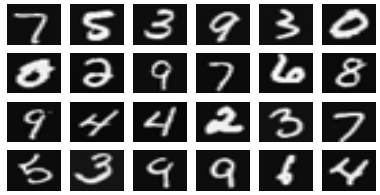
\includegraphics[width=0.7\textwidth]{images/handwritten_digits_example.png}
  \end{center}
  \caption{Example of $20 \times 20$ handwritten digits \cite{handwritten_digits_intro}.}
  \label{fig:handwritten_ex}
\end{wrapfigure}

One of the most effective solutions would be to provide our algorithm with large amount of such digits images to tune parameters of adaptive model. Such a set of images is called training set and the stage is known as a training phase. In it also a common practice to preprocess images to reduce dimensionality. For example if we would assume that our algorithm must run in real-time, processing large amount of pixels would be computationally inefficient. One of the mostly used technique assumes that one should consider only some of the images features. Features should be quick to compute and represent information that varies between images, hence can be used to discriminate between them. It is worth stressing out that preprocessing stage is crucial for overall system accuracy.


\section{Types of Learning}
One can distinguish between 3 main approaches to the learning procedure: supervised, unsupervised and semi-supervised. Following paragraphs will discuss them briefly - just to grab the idea.

\begin{wrapfigure}{l}{0.4\textwidth}
  \begin{center}
    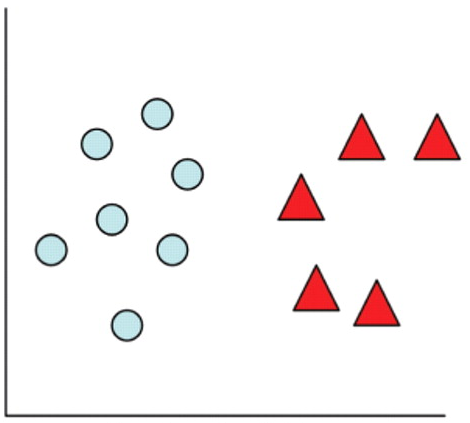
\includegraphics[width=0.55\textwidth]{images/supervised_graph.png}
  \end{center}
  \caption{Labeled data}
  \label{fig:handwritten_ex}
\end{wrapfigure}


\textbf{Supervised Learning} basically corresponds to processing data with a priori knowledge about its types. As in example from previous section, one is in possession of knowledge about types of digits. As said before algorithm must label input data as one of the following digits: 0, 1, 2, 3, 4, 5, 6, 7, 8 or 9. No other types are considered and all are known, hence the example is of supervised type. One can distinguish two approaches, based on type of input data:
\begin{itemize}
  \item Classification - assign discrete input data to discrete categories
  \item Regression - assign continuous input data to discrete categories.
\end{itemize}

\begin{wrapfigure}{l}{0.4\textwidth}
  \begin{center}
    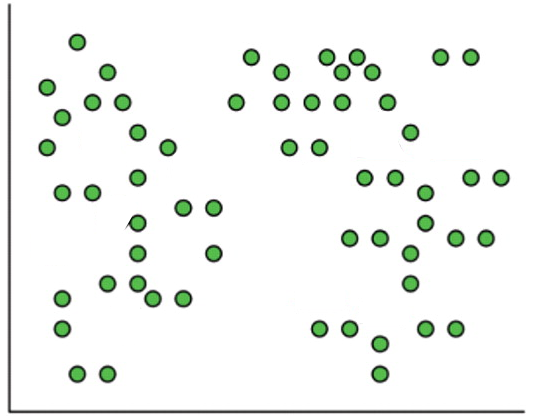
\includegraphics[width=0.55\textwidth]{images/unsupervised_graph.png}
  \end{center}
  \caption{Unlabeled data.}
  \label{fig:handwritten_ex}
\end{wrapfigure}

\textbf{Unsupervised Learning} copes with problems where there is lack of data labeling. We would for example consider our leading example as unsupervised if algorithm would be supplied only with pixel vectors with no associations to numbers they representing. The goal of unsupervised algorithm may vary from case to case, but can generally it considers following problems:

\begin{itemize}
  \item Clustering - discovering group of similar objects within data.
  \item Density Estimation - determine distribution over input space.
  \item Visualization - project from high-dimensions data to three dimensions, for the purpose of visualization
\end{itemize}

\begin{wrapfigure}{l}{0.4\textwidth}
  \begin{center}
    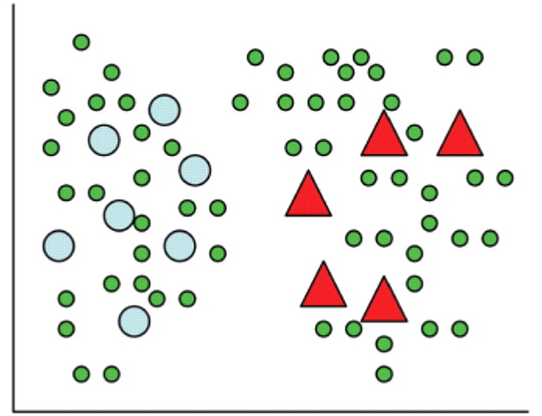
\includegraphics[width=0.55\textwidth]{images/semi_supervised_graph.png}
  \end{center}
  \caption{Labeled and unlabeled data.}
  \label{fig:handwritten_ex}
\end{wrapfigure}

\textbf{Semi-Supervised Learning} The goal of semi-supervised learning is to understand how combining labeled and unlabeled data may change the learning behavior, and design algorithms that take advantage of such a combination \cite{semi_supervised}. Often label instances are difficult, expensive, or time consuming to obtain, as they require the efforts of experienced human annotators. Because semi-it requires less human effort and gives higher accuracy, it is of great interest both in theory and in practice \cite{semi_supervised2}.


%-------------------------------------------------------------------
\pagebreak
\paragraph{}
\subsection{Quality Evaluation}\label{evaluation}
For better understanding of how quality of classification should be measured we adopt parameters and quality measures used in signal detection theory. Since these parameters are widely utilized, we do not refer to original sources here. The following parameters were used in defining several measures outlining classification's quality. These parameters create so called confusion matrix, which is given in Table~\ref{tab:conf_matrix}. The parameters given in the matrix are numbers of elements of a~testing set which have the following meaning:
\begin{itemize}
  \item $TP$ - the number of elements of the considered class correctly classified to this class,
  \item $FN$ - the number of elements of the considered class incorrectly classified to other classes,  
  \item $FP$ - the number of elements of other classes incorrectly classified to the considered class,  
  \item $TN$ - the number of elements of other classes correctly classified to other classes (no matter, if correctly, or not).  
\end{itemize}  

\begin{table}[H]
\vspace{-9pt}
\centering
\begin{tabular}{|c|c|c|}
\hline
  & & \vspace{-6pt}\\
  & \hspace{12pt}Classification to the class\hspace{12pt} & \hspace{3pt}Classification to other classes\hspace{3pt} \\
  & & \vspace{-6pt}\\
\hline 
  & & \vspace{-6pt}\\
  The class & True Positivse (TP) & False Negatives (FN) \\
  & & \vspace{-6pt}\\
\hline
  & & \vspace{-6pt}\\
  \hspace{3pt}Other classes\hspace{3pt} & False Positives (FP) &  True Negatives (TN)\vspace{3pt}\\
\hline
\end{tabular}
\vspace{9pt}
\caption{Confiusion matrix for rejecting in pattern recognition problem}
\label{tab:conf_matrix}
\end{table}

The following measures were used assess the quality of the classifier:
%\begin{flalign}
\begin{eqnarray}
  \textnormal{Accuracy}    & = &   \displaystyle\frac{\textnormal{TP+TN}}{\textnormal{TP+FN+FP+TN}}\nonumber\\
  \textnormal{Sensitivity} &\;=\;& \displaystyle\frac{\textnormal{TP}}{\textnormal{TP+FN}}\nonumber\\
  \textnormal{Precision}   & = &   \displaystyle\frac{\textnormal{TP}}{\textnormal{TP+FP}}\nonumber\\
  \textnormal{F--measure}  &\;=\;& 2\cdot\frac{\mbox{Precision}\cdot\mbox{Sensitivity}}{\mbox{Precision}+\mbox{Sensitivity}}
\end{eqnarray}

The following comments help to understand remaining of characteristics:

\begin{itemize}
  \item Accuracy is the measure of the rejecting performance. This measure describes the ability to distinguish between native and foreign elements. Of course, the higher the value of this measure, the better the identification.
  \item Precision is the ratio of the number of not rejected native elements to the number of all elements (native and foreign) not rejected. Precision evaluates the rejection ability to separate foreign elements from native ones. The higher the value of this measure, the better ability to distinguish foreign elements from native ones.
  \item Sensitivity is the ratio of the number of not rejected native elements to the number of all native ones. This measure evaluates the rejection ability to identify native elements. The higher the value of Sensitivity, the more effective identification of native elements. Unlike the Precision, this measure does not evaluate the effectiveness of separation between native and foreign elements. The higher the value of this measure, the better ability to identify native elements.
  \item Precision and Sensitivity are complementary: increasing sensitivity can cause a drop in precision since, along with increasing the number of not rejected native elements, there might be more not rejected foreign ones. It is there to express the balance between precision and sensitivity since, in practice, these two affect each other. There exists yet another characteristic that combines them: the \mbox{F--measure}. The higher the value of this measure, the better balance between identification of native elements along with separation native elements from foreign ones.
\end{itemize}
It is worth to say that other measures characterizing rejection quality can be invented, cf.~\cite{Homenda_2014}, but they are derivations from defined above.  

%---------------------------------------------------------------
\chapter{Automata and Languages Introduction} \label{chap:lan_theory}

The content discussed thus far, presented pattern recognition as a general problem. This chapter is considered to be a bridge between the pattern recognition world and the automata and language theory. We propose a set of procedures which help in reducing the classical problem of classification into a language theory problem. By doing so, we will be able to benefit from the prosperous and established theory.

The chapter begins with elements and classes transformations into words and languages, respectively. Then, the theoretic idea of classification process is sketched and finally the classification automaton is proposed.

%---------------------------------------------------------------
%---------------------------------------------------------------
\section{Transformation}\label{sec:lan_theory_transf}
This section is devoted to explaining the process of transformation of abstract classes into languages. All feature vectors are assumed to be of the same dimensions.

%---------------------------------------------------------------
%---------------------------------------------------------------
%---------------------------------------------------------------
\subsection{Word Transformation}\label{sec:lan_theory_transf_word}

Let us consider a feature vector~$f = [c_{1},c_{2},\ldots,c_{m}]$ and an alphabet $\Sigma=\{a_{1}, a_{2}, \ldots, a_{r} \}$, where $|\Sigma|=r$.
The first step of transformation process will include transforming each feature into an alphabet symbol. Recall that different features may belong to different intervals. For that reason, all features need to be normalized to a common interval. For convenience, the normalized interval will be defined by the size of the alphabet, namely $c_{i} \in \langle 0 , r \rangle$. The details of normalization are presented later in this section.

Having the interval conveniently normalized, we can now easily define the transformation of a single feature to a symbol by partitioning the intervals into $r$ sub-intervals: $x_1, x_2,\ldots,x_r$. We can now easily translate feature $c_i \in x_{j}$ by assigning the corresponding symbol $a_{j}$.

Formally the transformation of a single feature is defined as follows:

\begin{equation*}
c_i \featureTransformationSymbol{\Sigma}
\begin{cases}
a_1 & \text{for } c_{i} \in  \langle 0 , 1) \\
a_2 & \text{for } c_{i} \in  \langle 1 , 2) \\
a_3 & \text{for } c_{i} \in  \langle 2 , 3) \\
&\makebox[\widthof{${}\rightarrow{}$}][c]{\vdots} \\
a_{r} & \text{for } c_{i} \in \langle r -1, |\Sigma|  \rangle
\end{cases})
\end{equation*}

Having completed the transformation of all features of a given feature vector, the next step includes concatenating all consecutive symbols to create a word defining the feature vector. Formally, we define the word transformation as: $f \featureTransformationWord{\Sigma} w$, where $w \in \Sigma^*$ 

        
\begin{example} {\bf Word Transformation}\\
    Let $\Sigma =\{a,b\}$ be the alphabet and $\featureNorm{f} = [c_{1},c_{2},c_{3}]$ be a feature vector with normalized features to interval $\langle 0,2 \rangle$.
    Let $c_{1}=0.6$, $c_{2} = 1.5$, $c_{3} = 1.9$.
    By applying the feature transformation for all features we get:
    \begin{center}
        $c_{1} \featureTransformationSymbol{\Sigma} a$,
        $c_{2} \featureTransformationSymbol{\Sigma} b$,
        $c_{3} \featureTransformationSymbol{\Sigma} b$.
    \end{center}
    Finally the concatenation of consecutive symbols yields a word defining the feature vector $\featureNorm{f} \featureTransformationWord{\Sigma} w = abb$.
\end{example}

The following section focuses on the normalization process and mathematical details of transformation.

%---------------------------------------------------------------
%---------------------------------------------------------------
%---------------------------------------------------------------
%---------------------------------------------------------------
\subsubsection{Normalization} \label{sec:lan_theory_word_transf_norm}
One of the first challenges that appears during tackling the problem is features vector coding. By coding we understand changing vectors of real numbers into words over some alphabet. In case when the application has been supplied by real data, program needs to load tables and interpret them somehow. Following subsection describes process in general using mathematical description.

First of all let us assume that file has been already loaded and we are provided with set of features vectors: 

\[ F = \{ f_1 , f_2, \cdots , f_n \} \]

where each $f_i \in \mathbb{R}^{1 \times m}$, for $i \in \langle 1,n \rangle$.
Next we assume that set of $m$ features 

\[ C = \{ c_1 , c_2, \cdots , c_m \}\] 

has been supplied as well. With this knowledge we represent each vector from set $F$ as: 

\begin{align*}
f_1 = [ c_{11} \; c_{12} \; \cdots \; c_{1m}] \\
f_2 = [ c_{21} \; c_{22} \; \cdots \; c_{2m}] \\
\cdots \\
f_n = [ c_{n1} \; c_{n2} \; \cdots \; c_{nm}] 
\end{align*}

where entries of each vector represents values for consecutive features $c_1, c_2 \cdots , c_m$. We will use $c_{ij }\in f_i$ notation to refer to $j$th element of feature vector $f_i$

Since each feature from $C$ can take values from different intervals we decided to normalize all of them. There are two functions which will be useful in this process:
\begin{align*}
max : \{c_1, c_2, \cdots, c_m\} \rightarrow \mathbb{R} \\
min : \{c_1, c_2, \cdots, c_m\} \rightarrow \mathbb{R}
\end{align*}
Given feature $c_j$ for $j \in \langle 1, m \rangle$, they specify upper and lower boundary of the interval within which $c_j$ is captured. For example if $c_3$ takes values from interval $\langle -1 , 5 \rangle$, $max(c_3) = 5$ and $min(c_3 = -1)$.

Recall that $\Sigma$ represents an alphabet. Let us assume that $\Sigma = \{a_1 , a_2, \cdots, a_{|\Sigma|}\}$. Our goal is to hold all values of features vectors in $\langle 0 , |\Sigma| \rangle$ interval. To perform such conversion we will use following operation:
\begin{equation}
Intervals(f_i) \Leftrightarrow (\forall{c_{ij} \in f_i})(c_{ij} =  \frac{c_{ij} - min(c_{ij})}{max(c_{ij}) - min(c_{ij})} * |\Sigma|)
\end{equation}

for $i \in \langle 1, n \rangle$,$j \in \langle 1, m \rangle$ and $Intervals : \mathbb{R}^{1 \times m} \rightarrow \mathbb{R}^{1 \times m}$. Applied to each member of $F$, operation will force all feature vectors entries to be in $\langle 0 , |\Sigma| \rangle$ interval. Since we can easily split this interval to $|\Sigma|$ subintervals:

\[
\langle 0 , |\Sigma| \rangle = \langle 0 , 1) \cup \langle 1 , 2 ) \cup \langle 2 , 3 ) \cup \ldots \cup \langle |\Sigma| -2 , |\Sigma| -1 ) \cup \langle |\Sigma| -1, |\Sigma|  \rangle
\] 

following coding function can be defined:

\begin{equation}
Code(f_i) \Leftrightarrow (\forall{c_{ij} \in f_i})(c_{ij} = 
\begin{cases}
a_1 , \;\;\; c_{ij} \in  \langle 0 , 1)  \\
a_2 , \;\;\; c_{ij} \in  \langle 1 , 2 ) \\
a_3 , \;\;\; c_{ij} \in  \langle 2 , 3 )\\
\cdots \\
a_{|\Sigma|} , \; c_{ij} \in \langle |\Sigma| -1, |\Sigma|  \rangle\; 
\end{cases})
\end{equation}

for $i \in \langle 1, n \rangle$,$j \in \langle 1, m \rangle$ and $Code : \mathbb{R}^{1 \times m} \rightarrow \mathbb{R}^{1 \times m}$.

Now by performing:
\begin{equation}
(\forall{f_i \in F})(Code(Intervals(f_i))
\end{equation}
one will convert all features vector to words over $\Sigma$.

\begin{example} {\bf Normalization}\\
    Let us consider a feature vector where all features belong to original interval $\langle 0, 10 \rangle$, $f_1=[2, 6, 7]$. We will now apply transformation into a word over an alphabet $\Sigma=\{a,b\}$. Firstly the normalization process yields a normalized vector $\featureNorm{f_1}=[0.4, 1.2, 1.4]$. Finally $\featureNorm{f_1} \featureTransformationWord{\Sigma}w=abb$
\end{example}


%---------------------------------------------------------------
%---------------------------------------------------------------
%---------------------------------------------------------------
\subsection{Language Transformation}\label{sec:lan_theory_transf_lan}
Analogously to feature transformation, we will transform an entire class into a language over alphabet $\Sigma$.

Having an class $C$ with $n$ feature vectors: $f_1, f_2,\ldots,f_n$ one can transform it into a language $L$ by applying following language transformation: $C \featureTransformationLanguage{\Sigma} L_{C}$. The created language $L_{C} = \{w_1, w_2,\ldots,w_n\}$, contains words $w_i$ which have been constructed by transformation of corresponding feature vector $f_i \featureTransformationWord{\Sigma} w_i$. Thus language $L_{C}$ will look as follows:
\begin{center}
    $L_{C} = \{w \in \Sigma^{*} : \forall_{i} (f_{i} \in C, f_{i} \featureTransformationWord{\Sigma} w_{i}) \}$
\end{center}

Having an input set of classes: $C_{1},C_{2},\ldots,C_{m}$, where $C_{j}$ contains the feature vectors: $f_{j,1},f_{j,2},\ldots,f_{j,n}$, one can transform them into a set of languages. We assume that all feature vectors are of the same dimensions. Moreover, for simplicity of notation all classes are assumed to have the same number of elements, but it can be easily generalized for classes of different sizes. Applying the language transformation of a given alphabet $\Sigma$ we get the following set of languages:


\begin{align*}
&C_{1} \featureTransformationLanguage{\Sigma} L_{C_1} = \{w \in \Sigma^{*} : \forall_{i} (f_{1,i} \in C_{1}, f_{1,i} \featureTransformationWord{\Sigma} w_{1,i}) \} \\
&C_{2} \featureTransformationLanguage{\Sigma} L_{C_2} = \{w \in \Sigma^{*} : \forall_{i} (f_{2,i} \in C_{2}, f_{2,i} \featureTransformationWord{\Sigma} w_{2,i}) \} \\
&C_{3} \featureTransformationLanguage{\Sigma} L_{C_3} = \{w \in \Sigma^{*} : \forall_{i} (f_{3,i} \in C_{3}, f_{3,i} \featureTransformationWord{\Sigma} w_{3,i}) \} \\
&\makebox[\widthof{${}C_{1}xxxxxxxxxxxxxxxxxxxxxxxxxxxxxxxxxxx{}$}][c]{\vdots} \\
&C_{m} \featureTransformationLanguage{\Sigma} L_{C_m} = \{w \in \Sigma^{*} : \forall_{i} (f_{m,i} \in C_{m}, f_{m,i} \featureTransformationWord{\Sigma} w_{m,i}) \}
\end{align*}

The above transformation allows us to establish classification of a given element to a class in terms of words and language. Namely, if for the element $f$ the following transformation holds place:
\begin{center}
   $f \featureTransformationWord{\Sigma} w \in L_{C_3}$
\end{center}
then we can conclude that $f \in C_{3}$.

It is important to consider words that do not fall into any of the transformed languages. Such words will be rejected and thus considered to be foreign. The language containing all such words will be called a Foreign Language $L_{F}$. The language $L_{F}$ can be thought of as a special transformed language which includes all the remaining words that have not been created from transforming native classes.

%---------------------------------------------------------------
%---------------------------------------------------------------
%---------------------------------------------------------------
\subsection{Transformation Analysis}\label{sec:lan_theory_transf_prec}

Notice that the length of constructed word is equal to the size of feature vector. However, more importantly, the size of alphabet contributes in the accuracy of how well the word actually defines its corresponding feature vector. Consider the worst case scenario in which the alphabet contains only one symbol, $\Sigma=\{a\}$. Thus, transforming any feature vector $f$ of length $n$ will create the same word: $f \featureTransformationWord{\Sigma} w = a^{n}$


\begin{example} \label{ex:transf_prec}
    Let us consider two feature vectors where all features belong to original interval $\langle 0, 10 \rangle$, $f_1=[9, 5, 7]$ and $f_2=[5,9,7]$. We will now apply word transformation for both vectors for two different alphabets: $\Sigma=\{a,b\}$ and $\Gamma=\{a,b,c,d,e,f\}$. Applying the transformation for the first alphabet we get two words: 
    
    \begin{center}
        \begin{align*}
        &\featureNorm{f_1} \featureTransformationWord{\Sigma} w_1 = bbb, \\ &\featureNorm{f_2} \featureTransformationWord{\Sigma} v_1 = bbb.
        \end{align*}
    \end{center}
    
    Transformations for second alphabet yield: 
    
    \begin{center}
        \begin{align*}
        &\featureNorm{f_1} \featureTransformationWord{\Gamma} w_2 = fde, \\ &\featureNorm{f_2} \featureTransformationWord{\Gamma} v_2 = dfe
        \end{align*}
    \end{center}
\end{example}

The above transformation for the alphabet $\Sigma$ shows that for two seemingly distinct feature vectors we obtained two equal words. However, by applying transformation for bigger alphabet we managed to construct two distinguishable words.
it clearly visible that alphabet with higher amount of symbols will transform feature vectors into more precise word representations. Although, by increasing the size of the alphabet one has to expect higher time complexity of constructing the classifier.

In the example~\ref{ex:transf_prec} two different feature vectors have been transformed into the same word. This means that a word can belong simultaneously to more than one language. Thus in such a case:
\begin{center}
    $L_{1} \cap L_{2} \cap L_{3} \cap \ldots \cap L_{m} \neq \emptyset$
\end{center}

%---------------------------------------------------------------
%---------------------------------------------------------------
%---------------------------------------------------------------
\subsection{Language Similarity}\label{sec:lan_theory_lan_sim}
One could consider calculating transformation precision by determining how similar the languages are to each other.

Firstly, we must define word similarity. Two words can be thought to be \textit{similar} if the ratio of the length and their Hamming distance is reasonably small. Formally the similarity function of two words is defined by the equation:

\begin{definition} {\bf Word Similarity}
    \begin{equation}
    \wordSim{w}{v} = 1 - \frac{H_d(w,v)}{k}
    \end{equation}
    where $H_d$ is the Hamming distance and $k$ is the length of both words.
\end{definition}

Consider two words~$w~=~10101$~and~$v~=~00101$. The similarity $\wordSim{w}{v}$ is then equal to $0.8$.

Similarity of language $L_{1}$ to language $L_{2}$ is defined as follows. For word $w \in L_{1}$ calculate the maximum value of word similarity between $w$ and all words from $L_{2}$. Repeat for all words in $L_{1}$, averaging the results from all such words.

\begin{definition} {\bf Language Similarity\\}
The similarity of language $L_{1}$ to language $L_{2}$ is defined by the following equation:
    \begin{equation}
    \lanSim{L_{1}}{L_{2}} = \frac{1}{|L_{1}|} \sum_{w \in L_{1}} \max_{\forall_{v \in L{2}}} \wordSim{w}{v}
    \end{equation}

\end{definition}

The proposed Language Similarity is a asymmetric measure. Meaning that one language can be more similar to another than vice versa. It is an important feature when considering languages of different sizes. Consider two languages $L_{1}$ and $L_{2}$, where $L_{1} = \{w,v,u\}$ and $|L_{2}| = 50$.
If the word $w$ is added to $L_{2}$ then the similarity $\lanSim{L_1}{L_2}$ will raise very rapidly. On the other hand, the similarity $\lanSim{L_2}{L_1}$ will not be affected as much due to the large size of $L_{2}$.

%---------------------------------------------------------------
%---------------------------------------------------------------
%---------------------------------------------------------------
\subsection{Summary}\label{sec:lan_theory_transf_summary}
The method of class to language transformation has been introduced. The features have been transformed into alphabet symbols, elements into words and finally classes into languages. Moreover, the transformation process is based on the chosen alphabet, which size defines the transformation precision. Low precision of transformation can lead to improper classification while higher increased the computational time of constructing the classifier.

Additionally this section defined a way of describing classes in terms of languages. Languages $L_{C_1},L_{C_2},\ldots,L_{C_m}$ will commonly denote transformed languages representing their respective classes. The Foreign Language $L_{F}$ is the language of all other words which define elements that are considered to be foreign.

From now on, the fact that a word $w$ belongs to a language $L$, $w\in L$ will be used interchangeable with the fact that $w$ has been classified to a classes represented by $L$.

%---------------------------------------------------------------
%---------------------------------------------------------------
\section{Classification Language}\label{sec:lan_theory_class_lan}
Thus far, the method of classifying an element in terms of languages has been defined. This section focuses on the details of the classification process.

In the previous section it was mentioned that to properly classify a word to its language, it should be included in that language and should not appear in any other. In other words, the goal in proper classification should be the optimum partitioning of set of all words over alphabet $\Sigma$. The following explains the meaning of optimum partitioning.

%---------------------------------------------------------------
%---------------------------------------------------------------
%---------------------------------------------------------------
\subsection{Optimum Partitioning}\label{sec:lan_theory_class_lan_opt_part}

Recall from definition~\ref{def:myhill} that relation $R_L$ induced by the language $L$ partitions the set of all words $\Sigma^{*}$ into equivalence classes. In other words, equivalence classes are disjoint sets of words. Thus having an equivalence class which classifies a word to its respective language, could make for a very convenient classification tool.

Let the languages $L_{1}, L_{2} \text{ and } L_{3}$ be obtained from the language transformation. The idea of optimum partitioning is to split all three languages so that they are included in three different equivalence classes. 

The initial, poor, partitioning is illustrated in figure~\ref{fig:eq_classes_small_precision}. The figure presents example of three equivalence classes from possibly many. The language $L_{3}$ is fully and uniquely included in the class $A_{3}$. Language $L_{1}$ partially belongs to all three classes and $L_{2}$ belongs to both $A_{2}$ and $A_{3}$. Moreover, the first issue that should be addressed is the imperfect transformation precision. Namely, the intersection of languages $L_{1}$ and $L_{2}$ is not empty.

\begin{figure}[H]
    \centering
    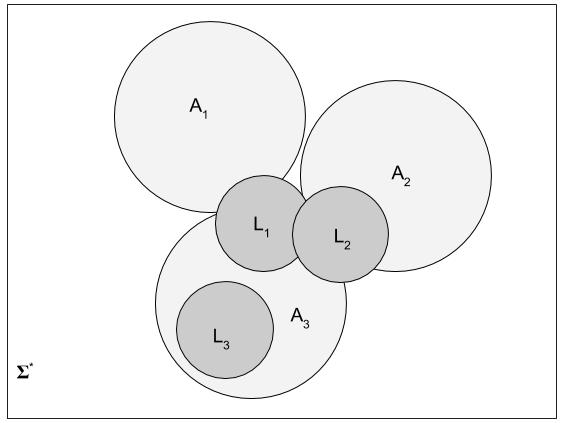
\includegraphics[width=0.5\textwidth]{./images/equivalence_classes_small_pt.jpg}
    \caption{Example of three equivalence classes of Relation Induced by the Classification Language. Languages overlapping and spread among multiple Equivalence classes}
    \label{fig:eq_classes_small_precision}
\end{figure}

Figure~\ref{fig:eq_classes_high_precision} shows the same partitioning for higher transformation precision. At this point, all three languages are disjoint but they also share a common class $A_{3}$. Assume that words that fall into $A_{1}$ are considered to be classified to $L_{1}$, similarly with $A_{2}$ for $L_{2}$ and $A_{3}$ for $L_{3}$. Thus having the languages included only partially in their respective classes make for a possible error in classification.

\begin{figure}[H]
    \centering
    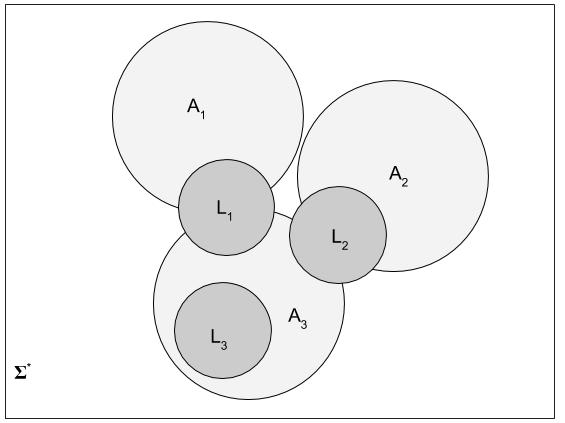
\includegraphics[width=0.5\textwidth]{./images/equivalence_classes_high_pt.jpg}
    \caption{Example of three equivalence classes of Relation Induced by the Classification Language. Languages are spread among multiple Equivalence classes}
    \label{fig:eq_classes_high_precision}
\end{figure}

The next improvement of partitioning is presented in figure~\ref{fig:eq_classes}. All languages are included in only their own respective classes. Words included in class $A_{1}$ will be classified to $L_{1}$. Thus in such a partitioning if words from $L_{1}$ were to be classified to $A_{1}$ then they would be necessarily classified correctly. The same applies to the other two languages. Although, a problem arises when words being classified belong to no particular language and thus are foreign. To maintain good quality of classification process, these words are not supposed to be classified to any of the three equivalence classes. Unfortunately, the classes might be very big, in fact, much bigger than the languages. Thus there are possibly many words that do not describe any particular object, which might be incorrectly classified as one. 

\begin{figure}[H]
    \centering
    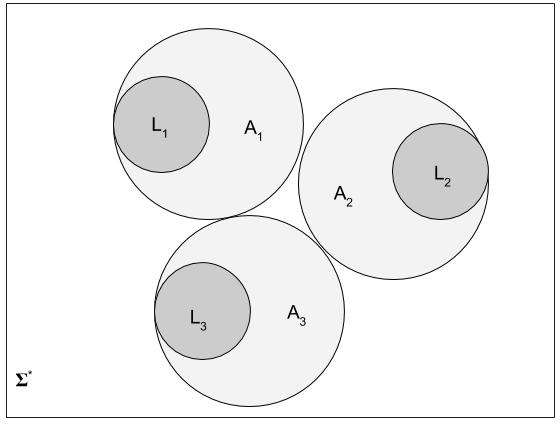
\includegraphics[width=0.5\textwidth]{./images/equivalence_classes.jpg}
    \caption{Example of three equivalence classes of Relation Induced by the Classification Language. Languages included in their respective equivalence classes}
    \label{fig:eq_classes}
\end{figure}

Finally, the figure~\ref{fig:eq_classes_ideal} presents the example of ideal partitioning for three languages. The space of classes and languages are equal, thus all words will be correctly classified.

\begin{figure}[H]
    \centering
    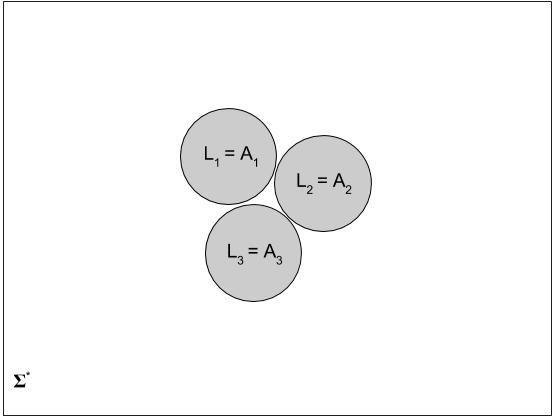
\includegraphics[width=0.5\textwidth]{./images/equivalence_classes_ideal.jpg}
    \caption{Example of three equivalence classes of Relation Induced by the Classification Language. Languages equal to their respective equivalence classes}
    \label{fig:eq_classes_ideal}
\end{figure}

In theory, the problem of optimum partitioning is a problem of constructing a regular language called Classification Language, $L_{C}$ for which equivalence classes of relation induced by $L_{C}$ contain the transformed languages. Ideally, each equivalence class which include and be equal to a single transformed language. The remaining classes will them correspond to the Foreign Language $L_{F}$. 

In practice equivalence classes might be very big and finding ones that perfectly describe a single transformed language can turn out to be a difficult task. Instead, a transformed language could correspond to few equivalence classes, although each class would still correspond to a single language. The intuition behind such procedure is to spread out the transformed languages across the space of all equivalence classes.

%---------------------------------------------------------------
%---------------------------------------------------------------
%---------------------------------------------------------------
\section{Classification Automaton}\label{sec:lan_theory_class_lan_dfa}

The Classification Language is a regular language and thus there exists a Deterministic Finite Automaton (DFA) which accepts it. Moreover, the states of such DFA correspond to the equivalence classes of relation $R_{L_{C}}$. DFA computes a word by returning a final state in which it stopped after the last symbol. Thus, now it is possible to built a classifier using merely a single DFA.

The figure~\ref{fig:class_dfa} shows an example automaton which is used to classify words. It is a deterministic finite automaton with four states and two symbols in the alphabet. States correspond to specific transformed languages. State $4$ corresponds to Foreign Language. Let us assume that some feature vector has been transformed into a word: $f \featureTransformationWord{\Sigma} w = bbb$. Computations for word $w$ will end in state $4$ and will be classified as foreign. However if $w = baba$ then the computations will end in state $2$ and the word will be classified to represent an object described in language $L_2$. Notice, that language $L_1$ is included in two states, in other words there are two equivalence classes that include $L_1$.

\begin{figure}[H]
    \centering
    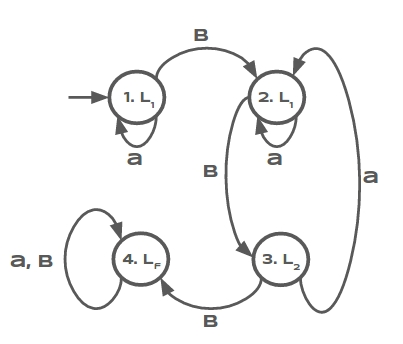
\includegraphics[width=0.7\textwidth]{../uml/states/dfa.jpg}
    \caption{Example of DFA with four states and two symbols. State 1 is the initial state. States $1$ and $2$ correspond to language $L_{1}$, state $3$ to $L_2$ and state $4$ to foreign language $L_F$.}
    \label{fig:class_dfa}
\end{figure}

Finally, building a proper classifier will be equivalent to creating an Classification Automaton $M_{C}$ that minimizes the error of classifying objects in the learning phase. The problem of choosing an optimal number of states corresponding to a transformed languages is to be parametrized and tested empirically.


%---------------------------------------------------------------
\chapter{Particle Swarm Optimization}\label{chap:pso}

The Particle Swarm Optimization (PSO) is population based stochastic optimization algorithm, originated by Eberhart and Kennedy~\cite{pso_origin}. Swarm of particles fly through the search space in order to find the most optimal solution of a given problem. The particles remember the best found solution and the further search is affected by it.

Each particle consists of the several fields. The position $X_p$ and velocity vector $V_p$ lets the particle travel through the search space. $Fitness$ value which is evaluated by the fitness function, represents the quality of the solution. The particle also remembers the best fitness value computed so far. Finally, two additional positions called $pbest_p$ and $lbest_p$ are stored. The position in which the particle $p$ reached its best fitness value so far is called $pbest_p$. However, the $lbest_p$ is the position of the best fitness value obtained so far by any other particle in the neighbourhood of particle $p$. The concept of neighbourhood is defined later in this chapter.

PSO is initialized with random group of particles. It then searches for the optimal solution by updating positions of the particles.
In each iteration $t$, the particles are updated by calculating potentially new $pbest_p$ and $lbest_p$ positions which affect the change in current velocity of the particle. $X_p(t)$ will denote the position of particle $p$ at time $t$, i.e. the $t$-th iteration. Similarly, the velocity vector is denoted by $V_p(t)$.

Firstly, the general flow of the PSO algorithm is given, then each functionality is discussed and defined in details.

\begin{center}
    
    \begin{enumerate}
        \item For swarm size s, initialize the group of particles.
        
        \item For each particle: \label{itm:pso_iter}
        \begin{enumerate}
            \item Calculate the fitness value, using the fitness function.
            \item Compare the fitness to its best obtained so far, the better value is stored together with $pbest_p$	
            
            \item Update neighbourhoods and find $lbest_p$ position.
            
            \item Update velocity and position.	
        \end{enumerate}
        
        \item Repeat~\ref{itm:pso_iter}. until maximum number of iterations has been reached.
        
    \end{enumerate}
    
\end{center}



%The remaining part of this chapter is devoted to illustrating problems associated with the objective of this study and more importantly, methods of solving these problems.


%---------------------------------------------------------------------
%---------------------------------------------------------------------
\section{Swarm Initialization}
In order to initialize the PSO algorithm, one must first decide on the size of the swarm (i.e. the number of particles). The swarm will be a static group, meaning that the size will not change through out the computations of a single PSO instance.

The interval for position of all particles must also be chosen. The interval along with the size of the position will essentially define the search space for the swarm.

Additionally, it is convenient to define a constant $v_{max}$ which prevents the particle from traveling in any dimension, further than $v_{max}$ distance in a single iteration. If the velocity was not limited, the jumps in position between iterations could be quite big. This could lead the particles to avoid a big chunk of the search space.


%---------------------------------------------------------------------
%---------------------------------------------------------------------
\section{Neighbourhood}

The neighbourhoods are updated using a simply algorithm based on star topology.
For each particle, neighbourhood is created containing itself and $K$ other random particles. Among that neighbourhood the best particle is found which defines the $lbest$ of the particle in interest.

The neighbourhoods are updated only when there was no change in global best (among all particles in the swarm) since the last iteration.


%---------------------------------------------------------------------
%---------------------------------------------------------------------
\section{Updating the particle}


The following method of updating the particles has its origins in the Standard Particle Swarm Optimization version 2011 presented in~\cite{pso_11}

Let $G_p(t)$ be the centre of gravity of the three points:
\begin{enumerate}
    \item Current position. \\
    $X_p(t)$
    
    \item Point a bit beyond $pbest_p$. \\
    $Y_{p1}(t) = c(pbest_p-X_p(t))$
    
    \item Point a bit beyond $lbest_p$. \\
    $Y_{p2}(t) = c(lbest_p-X_p(t))$
    
\end{enumerate}

The constant $c = \frac{1}{2} + ln(2)$ called a learning factor, together with the inertia parameter that weights the particle's velocity $\omega = \frac{1}{2 * ln(2)}$ used in further equations, was proposed by Clerc in~\cite{pso_anal}.

Formally $G_p(t)$ it is defined by the following formula 
\begin{equation}
    G_p(t) = \frac{X_p(t) + Y_{p1}(t) + Y_{p2}(t)} {3}
\end{equation}

We now define a random point $X^{'}_p$ in the hypersphere
\begin{center}
    $\mathcal{H}_p(G_p, d(G_p, X_p))$ 
\end{center}
of centre $G_p$ and of radius $d(G_p, X_p)$ where the function $d$ is an euclidean distance between two points. The time $t$ has been omitted for simplicity.

The velocity update is computed by
\begin{equation}
    V_p(t+1) = \omega  V_p(t) + X^{'}_p(t) - X_p(t)
\end{equation}
Thus the position is updated by the equation

\begin{equation}
    X_p(t+1) = \omega  V_p(t) + X^{'}_p(t)
\end{equation}

Figure~\ref{fig:pso_sphere} illustrates the idea of updating the position.

\begin{figure}[H]
    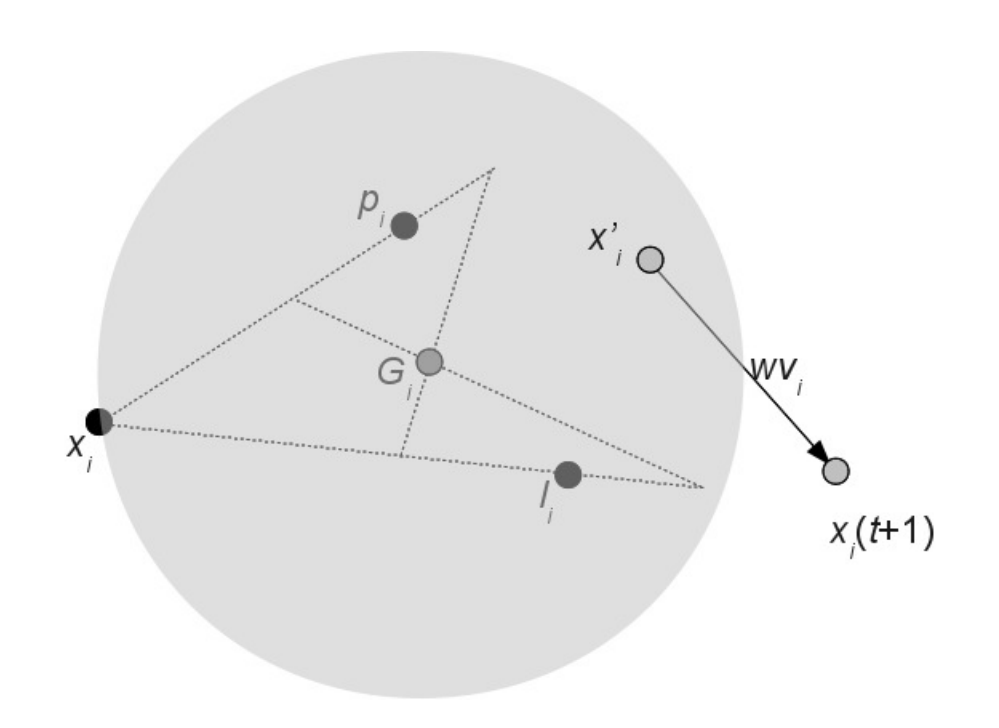
\includegraphics[width=0.7\textwidth]{./images/pso_sphere.png}
    \caption{Example of sphere  $\mathcal{H}_p(G_p, d(G_p, X_p))$. Point $x^{'}_{i}$ is chosen randomly within the sphere}
    \label{fig:pso_sphere}
\end{figure}

% Interval confinement
It may happen that the particle might leave the search space, in means that the particle lies outside the acceptable interval. If that happens we generally try to lead the particle back to its right course. For each dimension $x_{d} \in X_p$ that lies  outside the acceptable interval we apply the following:

\[
x_{d} \notin [x_{min}, x_{max}] \Rightarrow \left \{
\begin{array}{ll}
v_{d} = 0 \\
x_d < x_{min} \Rightarrow x_d = x_{min} \\
x_d > x_{max} \Rightarrow x_d = x_{max}
\end{array}
\right.
\]

This means that the corresponding dimension of velocity vector $v_d \in V_p$ is zeroed and the position is bound to the edge of the interval.

\section{Applying PSO}
In order to implement PSO for problem of interest, one must provide specific implementation for two major components of the algorithm. The first one is fitness function which optimizes the solution to a certain goal. The second one is particle representation method allowing to decode the particle into a specific object which can then be used in the fitness function.


%---------------------------------------------------------------
\chapter{Hill Climbing}\label{chap:hill_climbing}

% Funny quote 
\epigraph{'' ... (Hill Climbing) resembles trying to find the top of Mount Everest in a thick fog while suffering from amnesia. ''}{\textit{Stuart Russell \\ Peter Norvig }}

\bigskip

% Intro - what is it etc
The hill-climbing search algorithms, also known as 1+1 evolutionary strategies \cite{hc_1}, are the simplest form of evolutionary algorithm, but often perform competitively with more complex evolutionary algorithms \cite{hc_2}. It is simply a loop that continually moves in the direction of increasing value-that is, uphill. It terminates when it reaches a "peak" where no neighbor has a higher value. The algorithm does not maintain a search tree, so the current node data structure need only record the state and its objective function value. Hill-climbing does not look ahead beyond the immediate neighbors of the current state \cite{hc_3}.

\begin{wrapfigure}{l}{0.25\textwidth}
    \begin{center}
        
\includegraphics[width=0.8\textwidth]{./images/hc_1.png}
    \end{center}
\end{wrapfigure}

% Motivation - WHY ?!
Choosing Hill Climber (HC) as an alternative to previously described Particle Swarm Optimization (PSO), was mainly driven by a desire of comparison between sophisticated heuristic and something more straight forward. Previous optimization method assumed rather convoluted process of finding solution, whereas HC is based on small and easy steps which gradually leads to (hopefully) optimal solution. As an evidence, one could consider lack of crossover operators. When in PSO constant change between real valued and DFA spaces was mandatory, Hill Climber performs all computations in the latter one. By few operations and data structures one can find fairly good (in terms of classifying) solutions in reasonable time. 

% General steps of hill climbers
\section{Basic Model}
Pseudo code listed as Algorithm \ref{algo:hc_general}, presents general process of Hill Climbing. Notation includes generic names to depicts the idea itself, rather than dive into some specific implementation. User is asked to specify two values: starting state $s$ and number of steps $n$. When the latter one is obvious, $s$ constitutes problem-related, starting configuration e.g. it can be opening positions of queens on chessboard in 8-queens problem or matrix representation of a graph for Traveling Salesman Problem. Then in lines 2 and 3, one can observe initialization process of two variables: $i$ (step counter) and $current$ (present state holder). Of course $current$ takes value of $s$ to force the procedure to start from a desired state. Core part of the algorithm is based on $while$ loop, which ends either when number of steps has been passed (line 4) or there is no neighbor with higher objective function around (line 6,7). \textsc{OBJ-FUNCTION} (objective function) resembles another abstract and problem-related procedure, which measures quality of a given state. As an example one can take beforementioned Traveling Salesman Problem, where objective function could result in specifying a route length for its input. 

\begin{algorithm}[H]
    \SetKwInOut{Input}{Input}
    \SetKwInOut{Output}{Output}
    \Input{Starting state $s$, number of steps $n$}
    \Output{Local optimum state.}
    \underline{function HILL-CLIMBING-BASIC} $(s, n)$\;
    $i = 0$ \\
    $current = s$ \\
    \While{$i < n$}
    {
        $neighbor$ $\gets$ a highest-valued neighbor of $current$ (in terms of objective function) \\
        
        \If{OBJ-FUNCTION[current] $\geq$ OBJ-FUNCTION[neighbor]}
        {
            \Return{current}
        }
        
        $current$ $\gets$ $neighbor$
    }
    \caption{General Hill Climbing Algorithm}
    \label{algo:hc_general}
\end{algorithm}

% Problems in state vs objective function space
It can be easily seen, that general model of HC is rather a basic one due to process of "giving up" when there is no better solution around. One can distinguish common topographic features in a searching space, which via they shapes, prevent general Hill Climbing procedure to achieve global optimum. To preserve transparent and abstract approach, figure \ref{fig:state_space} treats state space as a one dimensional. In addition any fluctuation of the graph correspond to values of objective function for a given state. 

\begin{wrapfigure}{l}{0.5\textwidth}
  \begin{flushleft}
     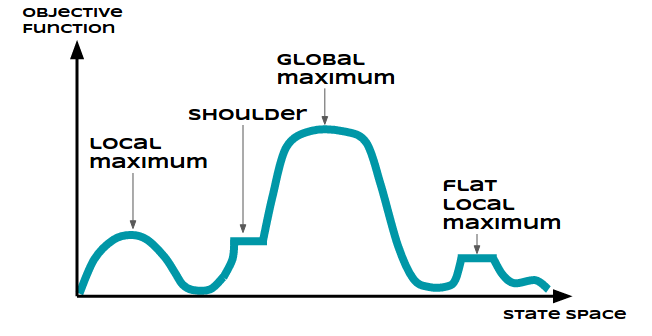
\includegraphics[width=1\textwidth]{./images/hp_landscape.png} 
  \end{flushleft}
  \label{fig:state_space}
  \caption{Landscape of state space.}
\end{wrapfigure}

Obviously, considering landscape presented on the image, global maximum is the place we want our travel to finish. One can easily spot that reaching the highest summit is simply impossible from various points on the landscape. As an example let us assume we are starting our journey from the origin. After short climbing HC would reach local maxima and stuck there due to lack of neighbors with higher values of objective function. Another example would be visiting the shoulder. At the very beginning of the ledge, algorithm would assume that there is no better neighbor (only ones with the same values) and would prevent further climbing to the global maxima. It is worth to notice that both, shoulder and flat local maximum, are often called plateaux, which corresponds to an area of the state space landscape where the evaluation function is flat \cite{hc_3}.

\section{Improving Basic Model} \label{sec:improving basic model}
% Improved HC
Most of the problems presented in the previous section can be easily omitted. Algorithm \ref{algo:hc_improved}, although at first glance similar to Algorithm \ref{algo:hc_general}, tackles the issues very effectively. 

First difference that can be easily spotted are randomly generated neighbors. They are normally drawn from the states space with uniform probability distribution and constitutes efficient way to escape from local optima. Let us consider figure \ref{fig:state_space} once again. As mentioned before, assuming that HC reached local maximum, algorithm in basic model would end. But this is not a case in the improved version, where HC could pick up random neighbor (e.g. from the slope of global maximum) with higher value of objective function and continue the computations. In this way we are only limited to a number of steps i.e. there is no way to get out of the \textsc{while} loop different than using up all steps. Such approach actually introduces new problem - when one is dealing with large multidimensional states space, there might be a lot of steps needed to even a little bit elevate objective function. 

Second improvement deals with plateaux. It simply assumes that when considered neighbor has the same (or higher) value as a current state, then we mark the neighbor as a current state and continue. In this way, Hill Climbing would travel across e.g. shoulder or flat local maximum. Such movement is often called sideways move. It may be interesting that applying only this improvement (without randomly generated neighbors) to the basic model, could result in infinite loop at flat local maxima. This is because algorithm would travel from one end of the ledge to the other, being limited only by a specified number of steps.

\begin{algorithm}[H]
    \SetKwInOut{Input}{Input}
    \SetKwInOut{Output}{Output}
    \Input{Starting state $s$, number of steps $n$}
    \Output{Local optimum state.}
    \underline{function HILL-CLIMBING-IMPROVED} $(s, n)$\;
    $i = 0$ \\
    $current = s$ \\
    \While{$i < n$}
    {
    	$neighbor$ $\gets$ randomly generated state, different than $current$ \\
    	
    	\If{OBJ-FUNCTION[neighbor] $\geq$ OBJ-FUNCTION[current]}
    	{
			$current$ $\gets$ $neighbor$
   		}
   		  		
    }
    \caption{Improved Hill Climbing Algorithm}
    \label{algo:hc_improved}
\end{algorithm}

At the end I would like to devote one paragraph to completeness of described methods. Basic and improved Hill Climbers, in literature called Steepest Ascent and First-Choice, respectively, often fail to find global optima. They usually stuck on local ones or do not have enough steps to find random neighbors with higher values of objective functions. Both of them along with Stochastic Hill Climbing (where uphill move is chosen at random from among all neighbors moves) constitute widely known and used approaches, which are not complete. For HC to become complete, one must consider Random-Restart Hill Climbing. This model conducts series of searches from randomly generates starting states. Obviously it is complete with probability reaching 1, due to the fact that eventually goal state would be generated as an initial one. It is also worth stressing out rather evident observation that success of HC models mostly rely on shape of the states space. In case of few local optima and/or plateaux all of them should find satisfiable solutions very quickly. 


\section{Hill Climbing and Automata} \label{sec:hc_automata__}

\begin{wrapfigure}[9]{l}[0pt]{0.3\textwidth}
  \begin{center}
    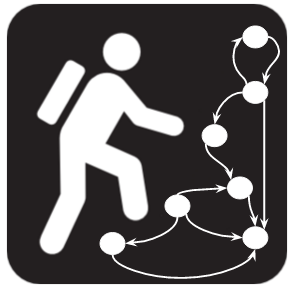
\includegraphics[width=0.7\textwidth]{./images/hc_auto_1.png}
  \end{center}
\end{wrapfigure}
This section will present general idea of adapting Improved Hill Climbing model to work with Deterministic Finite Automata. Step by step approach has been assumed, allowing reader to understand consecutive elements of the implementation. Work is a partial implementation of ideas from ??.

To start with, we would like to present a general overview of the process to give reader some insight about each part described further. Hill Climbing starts with some randomly generated automaton. At each step current automaton is compared with another one, built by randomly changing one of the transitions. If objective function for the new one is at least the same as for the current one - new become current. Objective function will be based on some training set of words and will check number of correct computations for each of them. Hill climbing will work until individual that perfectly fits the training set is found or number of step is exceeded.

\subsection{DFA Search Space}

\begin{wrapfigure}[9]{l}{0.4\textwidth}
  \begin{center}
    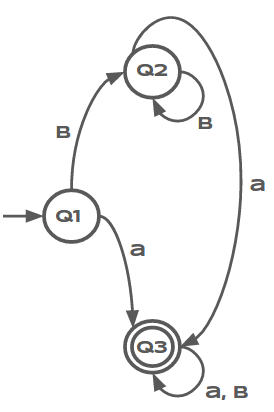
\includegraphics[width=0.7\textwidth]{./images/hc_automata.png}
  \end{center}
\end{wrapfigure}

Deterministic Finite Automata in case of hill climbing will be represented by two arrays:
\begin{itemize}
  \item Transition Table - states versus symbols:\\
  		\begin{minipage}[t]{\linewidth}
          \raggedright
          \adjustbox{valign=t}{%
            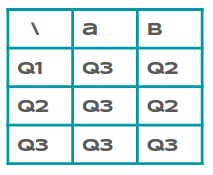
\includegraphics[width=.4\linewidth]{./images/hc_tt_normal.png}%
          }
    	\end{minipage}
  \item State Correspondence Array - represents states labeling, needed for further classification process. For simple two class problem, it marks states as either accepting or rejecting ones:\\
  \begin{minipage}[t]{\linewidth}
          \raggedright
          \adjustbox{valign=t}{%
            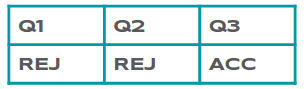
\includegraphics[width=.5\linewidth]{./images/hc_state_corr.png}%
          }
    	\end{minipage}
\end{itemize}
\bigskip
Combination of both, transition table and state correspondence array constitutes good candidate for a  hill climbing's state space. In this case number of possible combinations of these arrays with data is given by:
\begin{equation}
S = q^{q \sigma}c^{q}
\end{equation}
where $q$ represents number of states, $\sigma$ constitutes number of distinct symbols in the alphabet and $c$ is number of classes considered.

As an example let us take above automaton. It has three different states, alphabet is based on two symbols and it deals with two class problem (\textsc{REJ} or \textsc{ACC}). Number of all possible combinations for such automaton equals $S = 3^{2 \cdot 3}\cdot2^{3} = 5832$. Not much.

\subsection{Smart State Labeling} \label{subsec:smart_labeling}
Introduced in \cite{hc_4}, Smart State Labeling resembles a way to decrease search space by the factor of $c^{q}$, which comes from all possible combinations of State Correspondence Array. Authors introduced simple, yet novel approach to automatically assign classes to states at each step of the algorithm. They realized that during hill climbing, there will certainly exist some epistasis or dependency between transition matrix and states labeling.

Let $h[i][c]$ be an array denoting the number of times the DFA finished in state $i$ for pattern class $c$. We refer to set of training words as $T$ and all entries of $h$ are initialized to zero. In addition we say that $f(t)$ represents final state reached by element $t \in T$. Having all of that we can define the process of Smart State Labeling as a two step algorithm:
\begin{enumerate}
\item For all $t \in T$, representing class $c$, increment $h[f(t)][c]$.
\item For each state $i$, assign $\argmax_c h[i][c]$.
\end{enumerate}
In this way, the search space got reduced to $S = q^{q \sigma}$

To better understand the process let us present an example. Figure \ref{fig:smart_state_example} represents 3 consecutive steps of hill climbing with Smart States Labeling. Considered automaton has three states, two symbols and we are dealing with two class problem. In addition, set $T$ has ten elements. Figure \ref{fig:smart_state_example_1} represents initial step. Array $h$ has its entries set to zero and state correspondence has been chosen randomly. In the second step (Figure \ref{fig:smart_state_example_2}), one can observe that transition of the DFA has been randomly changed - now from state $Q2$ via symbol $b$ machine will lead to $Q1$. In addition $h$'s entries are set to values according to above algorithm. Because of that $Q3$ stopped, and $Q1$, $Q2$ started, being accepting states. Figure \ref{fig:smart_state_example_3} constitutes another example of an artificial step. Again we can observe change in a DFA's transitions along with states correspondence.

\begin{figure}[H]
\RawFloats
\centering
\begin{minipage}{.3\textwidth}
\centering
  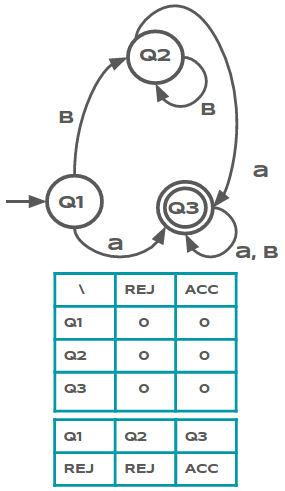
\includegraphics[width=0.8\textwidth]{./images/hc_example_1.png}
\caption{}
\label{fig:smart_state_example_1}
\end{minipage}\hfill
\begin{minipage}{.3\textwidth}
\centering
  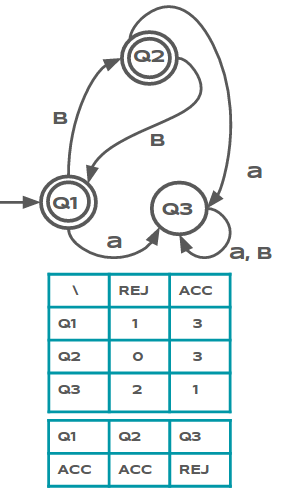
\includegraphics[width=0.8\textwidth]{./images/hc_example_2.png}
\caption{}
\label{fig:smart_state_example_2}
\end{minipage}\hfill
\begin{minipage}{.3\textwidth}
\centering
  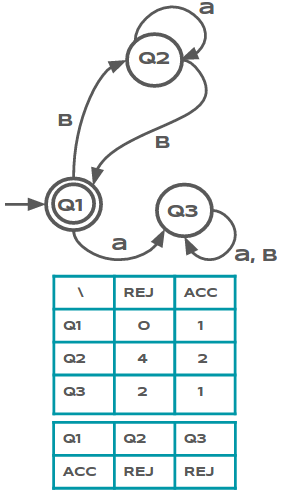
\includegraphics[width=0.8\textwidth]{./images/hc_example_3.png}
\caption{}
\label{fig:smart_state_example_3}
\end{minipage}
\label{fig:smart_state_example}
\caption{Example of 3 different steps of HC with Smart States Labeling. First image represents initial configuration, where next two are some steps from the algorithm computations.}
\end{figure}

\subsection{Objective Function} \label{subsec:obj_func}
In standard approach one would deal with different procedure for evaluating DFAs quality in consecutive steps of the algorithm, but in our case we will use $h$ for that purpose.

To directly compute objective function $F$, one should sum up biggest values of $c's$ for all states and divide it by a number of elements in set $T$ i.e.
\begin{equation}
F = \frac{\Sigma_{i=1}^{n} max_c h[i][c]}{|T|}
\end{equation}
In this way, ratio between number of correctly classified elements of training set and number of all elements of $T$ will be obtained. Obviously $F \in \langle 0 ; 1 \rangle$, and our goal is to obtain $F=1$.

\subsection{Algorithm} \label{subsec:algo_hc__}
At this stage we would like to gather previously presented ideas to forge the algorithm itself. Algorithm \ref{algo:hc_finial} represents final scheme of hill climbing with Smart States implementation.

\begin{algorithm}[H]
    \SetKwInOut{Input}{Input}
    \SetKwInOut{Output}{Output}
    \Input{Number of states $q$, number of symbols $\sigma$, number of classes $c$, training set $T$, number of steps $n$}
    \Output{Transition table of optimal DFA.}
    \underline{function DFA-HILL-CLIMBING} $(q, \sigma, c, T, n)$\;

    \bigskip
	$transitionTable[q][\sigma]$ $\gets$ randomize entries \\
	$states[c]$ $\gets$ randomize entries \\
    \bigskip

    \While{$i < n$}
    {
    	$valuePrev$ $\gets$ OBJ-FUNCTION($tranitionTable$, $states$) \\
		$temp$ $\gets$ one entry from transition table (value and position) that will be updated \\
		\bigskip

		$transitionTable[temp.position]$ $\gets$  random integer from interval $\langle 0 ; q \rangle$\\
		$statesCurrent$	$\gets$  SMART-STATES[$tranitionTable$, $T$]\\
		$valueCurrent$ $\gets$ OBJ-FUNCTION($tranitionTable$, $statesCurrent$) \\
		\bigskip

    	\eIf{$valueCurrent$ $\geq$ $valuePrev$}
    	{
			$states$ $\gets$ $statesCurrent$ \\
   		}
   		{
   			Restore value saved in $temp$ to $transitionTable$ \\
   		}
    	\bigskip
   		\If{$valuePrev$ $ = 1$ or $valueCurrent$ $ = 1$}
    	{
			\Return $transitionTable$ \\
   		}
   		$i \gets i + 1$
    }

    \bigskip
    \Return $transitionTable$ \\

    \caption{Hill Climbing Algorithm for learning a DFA.}
    \label{algo:hc_finial}
\end{algorithm}
\pagebreak
Following values are assumed as an input: number of states $q$, number of symbols $\sigma$, number of classes $c$, training set $T$, number of steps $n$. At the beginning initialization of $transitionTable$ and $states$ (States Correspondance Array) takes place. Both of them have randomized input. All random operations assumes uniform distribution.

Next the procedure start its main \textsc{WHILE} loop, with condition checking number of steps. At lines 5 and 6 we record the index of the transition that was mutated and the previous value of the transition and use this information to revert the change if a deterioration in objective function occurred. Such approach saves both time and space of the algorithm. During this procedure already known \textsc{OBJ-FUNCTION} is used. In our case its implementation is consistent with function $F$ described in details in section \ref{subsec:obj_func}. What is more variable $temp$ may be understand as a data structure, which saves three values: row index, column index and value.

When previous value has been saved, the algorithm continues to randomly modifies \\ $transitionTable$ (line 7) and calculating new value of objective function. \textsc{SMART-STATES} procedure assumes as an input transition table and training set. It returns new states correspondence array calculated using arguments and algorithm described in section \ref{subsec:smart_labeling}. Hence $statesCurrent$ represents DFA with transitions described by modified $transitionTable$. Finally \textsc{OBJ-FUNCTION} can be called and its value is saved for further comparison in variable $valueCurrent$ (line 9).

At this point comparison of both, current and newly generated DFA happens. If in line 10 occurs that fresh DFA works better, only thing that we need to do is save $statesCurrent$ in $states$ variable. Otherwise we need to restart $transitionTable$ to its original form. We do it by recalling values saved in $temp$.

Additional conditional statement is called at line 15, checking if any of calculated value has reached maximum (value of 1). If this happens Algorithm \ref{algo:hc_finial} ends its computations.

%---------------------------------------------------------------
\chapter{Classifier Construction}\label{chap:classifier}

In this chapter, each step of building the classifier is summarized and explicitly described.

%---------------------------------------------------------------
%---------------------------------------------------------------
\section{Transformation Analysis}
Even before selecting heuristic method, one must choose the alphabet size for transformation process. The transformation analysis will help in determining the optimal alphabet size. In this thesis the analysis was conducted separately from classifier construction and thus the alphabet was chosen empirically.

%---------------------------------------------------------------
%---------------------------------------------------------------
\section{PSO for Classification}
 
Applying PSO to the problem of automata optimization, requires a tool of evaluating the quality of an automaton. The following sections introduce the reader to the methods of turning the abstract PSO algorithm to the  automata optimization. Finally, PSO requires the selection of states which will correspond to languages. The correspondence is to be selected empirically. 

%---------------------------------------------------------------------
%---------------------------------------------------------------------
\subsection{Particle Decoding}


Particle decoding algorithm takes as an input number of states $n$ and number of symbols in the alphabet $r$.
Let us recall that automaton is a system: $A = (Q, \Sigma, \delta, q_0, F)$. In a single PSO instance we assume that a set of states $Q$ and alphabet $\Sigma$ is invariant. 

The position of our particles will be represented by the natural decoding vector of size $n*r$ of an automaton described in section~\ref{sec:auto_dec} with more freedom allowed. Namely, all of the dimensions of the position will take real values in the interval $[0.5, (n+0.5)]$. Whenever we need to encode the automaton back, we simply round up the values, taking the closest integer value. The real number $3.4$ becomes $3$ and $3.5$ becomes 4. Notice that the interval is expanded by the value $0.5$. Such procedure is needed to allow for equal distribution of the first and last states. Namely, the first state will be encoded for values: $[0.5, 1.5]$ and the last state: $[(n-0.5), (n+0.5)]$.

%---------------------------------------------------------------
%---------------------------------------------------------------
%---------------------------------------------------------------
\subsection{Fitness Function}

Fitness function is responsible for optimizing the classification automaton. In order to experiment with different optimization methods, 8 fitness functions have been proposed. The optimization functions are split into two categories: distinct and indistinct. The former one optimizes the classifier to identify between native classes individually (i.e. multi class classification). The indistinct one, considers native classes as one big class, and thus it treats the optimization as two class classification: native against foreign.

In each of the two categories, 4 functions based on the common classifier quality measures defined in section~\ref{evaluation} are proposed:
\begin{itemize}
    \item Accuracy Fitness
    \item Precision Fitness
    \item Sensitivity Fitness
    \item F-Measure Fitness
\end{itemize}

The fitness function must also be provided with the transformed languages and state correspondence. That is, it must know which state must correspond to a specific language. Then at each iteration, after the particle is decoded to automaton, all words are to be computed by the automaton and checked against the state correspondence. then the above measures will calculate the fitness value based on the classification quality. The higher the value of these measures, the better is the solution defined by the particle.

%---------------------------------------------------------------
%---------------------------------------------------------------
\section{HC for Classification}
There is no further work needed - Hill Climber, as described in section \ref{sec:hc_automata__} can be ad hoc used as a classifier. It accepts as its input set of training words and via algorithm, described in details in subsection \ref{subsec:algo_hc__}, builds and returns proper representation of a Deterministic Finite Automata. Such a DFA constitutes a classifier.


%---------------------------------------------------------------
\chapter{Experiments}\label{chap:experiments}
%%%%%%%%%%%
% WH

%Experiment is done on vectors of features, vectors represent images.
%Mapping from the set of images to the space of features to be described.

% WH/
%%%%%%%%%%

%%%%%%%%%%%
% WH

%- features vectors: are given by supervisor and cannot be used without written permission for any aim other than this thesis, put this information in footer

% WH/
%%%%%%%%%%

The datasets of vectors of features were constructed based on the MNIST database of handwritten digits~\cite{digits_db}. Sample of the original images is presented in figure~\ref{fig:native_foreign_png}. The upper image shows sample of original native elements. The foreign elements (bottom image) have been constructed from the native ones by crossing them out. The vector of features were constructed by extracting features from these images. All vectors contained $24$ features.

The native dataset contained $10$ classes, each representing different handwritten digits. Every class had $900$ vectors of features, totaling $9000$ across all native classes. The foreign data was considered as one class and contained $9000$ vectors of features. Finally each class has been divided into training($60\%$) and testing($40\%$) sets. Training set was used in the optimization process and testing set to calculate quality of the classifier.

\begin{figure}[H]
    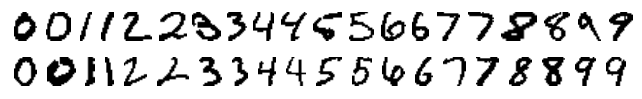
\includegraphics[width=0.7\textwidth]{./images/native.png}
    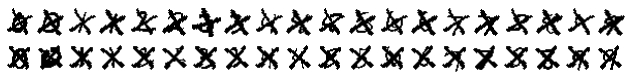
\includegraphics[width=0.7\textwidth]{./images/crossedout.png}
    \caption{From the top: Native and Foreign - crossed out digits.}
    \label{fig:native_foreign_png}
\end{figure}

The experiments are divided into two main categories: multi class and two class classification. In the former one, all native classes are considered individually. In the latter case, all native classes are combined into one big class. Thus it is a problem of distinguishing between native and foreign elements.

\section{Transformation Analysis}

Calculating the similarity of languages can potentially determine a correlation between alphabet size and the quality of constructed classifier. The similarity experiment will be done for both multi class and two class classifications. In the former one, the similarity will be computed between all native languages. In the two class classification, all native languages are to be combined into one big and its similarity will be checked against the foreign language. In each case the similarity computation will be ran for alphabet size in the interval: $[1,40]$.


\section{PSO}
The motivation behind these tests is to study the quality of classifier on different alphabet sizes as well as different state configurations. The four distinct fitness functions were used in the multi class optimization. Similarly the two class optimization was experimented using indistinct fitness functions. All experiments have been repeated $3$ times and the results were averaged. Additionally, the multi class classification is tested for different number of classes. 
\section{HC}
Fitness function, described (and referred to as objective function) in section \ref{subsec:obj_func} has been used in both, multi and two class optimization. All experiments have been repeated $3$ times and the results were averaged. Additionally, the multi class classification is tested for different number of classes.

%---------------------------------------------------------------
\chapter{Results}\label{chap:results}
\selectcolormodel{gray}

\section{Transformation Analysis}

The similarity between all native languages is shown in table~\ref{fig:tab_similarity}. Each row defines similarity of corresponding language to all other depicted in columns. For example, $\lanSim{L_0}{L_9} = 0.34$ and $\lanSim{L_9}{L_0} = 0.33$. Recall that introduced similarity measure is asymmetric. However, the similarities between transformed languages are nearly perfectly symmetric.

\makeTableMutualSimilarites

All of the similarities have been averaged and shown in figure~\ref{fig:lang_sim}. The averaged similarities have been computed for the range of alphabet sizes in the interval $[1, 40]$. In multi class the similarity have been computed between all 10 native languages. In two class, presented similarity is computed between one combined native language and the foreign one. Both scenarios have resulted with almost the same values. When the alphabet size is equal to $1$, then obviously the averaged similarity between languages is equal to $1$. Initially, the similarities grow quickly and stabilizes at alphabet size equal to approximately $30$. At this point the differences in similarities between consecutive iterations is very small. One could choose alphabet size of $30$ in order to keep a good balance between computational complexity and language similarities.

\makeFigureAvgSimlarity


\section{PSO}

Results of classifier construction based on PSO is presented in this section. The results for multi class optimization is shown first, then the discussion turns to two class.

\subsection{Multi Class}

The figure~\ref{fig:fitness_multi} shows results of the multi class classifier for four different fitness functions. In that case, the state configuration was not changed and included $20$ native states -- $2$ per class and $20$ foreign states. The computations were repeated for alphabet sizes: $10$, $30$ and $40$.

In all four cases, the classifier did not manage to correctly recognize between native elements, hence the low sensitivity values. Moreover, the accuracy was bellow $0.5$ across all test cases. 

In the case of Accuracy Fitness based optimization the best result was obtained with alphabet size equal to $30$. At this point, the precision was equal to $0.8$ which gives a reasonable result on distinguishing the foreign elements Although, most importantly, this function did not help in constructing accurate classifier. The Precision based optimization, had very similar results. Finally, the Sensitivity and F-Measure optimizations constructed extremely low quality classifier.

Next experiment included tests with different state configuration. The results are presented in figure~\ref{fig:states_multi}. Accuracy based optimization was used as the goal function, the alphabet size was fixed on $30$. In all four cases, each of the native classes corresponded to $2$ states, hence $20$ in total. The foreign class had: $10$, $20$, $40$ and finally $80$ states. In the first two configurations, results were the same. However, by increasing the number of states that govern foreign class we obtained lower precision. Together with the fact that accuracy value remained equal, one can conclude that many of the native elements were incorrectly classified as foreign. Moreover, we can see that the precision was already equal to $0.8$ when the number of foreign states was equal to the half of all natives, as it is depicted in the first test case. It might suggest that the foreign elements were all similar enough so that their class did not require to take up much space. To able to separate foreign elements from native, one should keep state configuration in balance.

\makeFigureFitnessMulti

\makeFigureStateConfigurationMulti

\makeFigurePSOClasses

Final experiment in the multi class optimization, tested the behavior of the classifier on different number of classes. In figure~\ref{fig:pso_classes} shows results of constructing classifiers with different number of included classes. In all cases, native classes corresponded to $2$ states and foreign had always as many as all natives combined. The alphabet size was fixed at $30$.

The overall quality got worse very quickly between $2$ and $3$ native classes. From that point, the classifier could not correctly classify native elements. However the precision remained relatively stable.

In all cases, only the required classes were loaded from both native and foreign data sets, meaning that transformation did not include the entire spectrum of provided feature values. The test merely gives an idea of how many classes can be supported by using the proposed algorithms.



\subsection{Two Class} \label{subsec:pso_two_class}

The discussion now turns into two class optimization, where all native classes are considered as one. Hence, all of the quality measures have been calculated accordingly.
The figure~\ref{fig:fitness_two} presents results for different optimization functions. The state and alphabet configurations remains the same as previously. The alphabet size had impact only in the case of Precision Fitness, where again $30$ seemed to yield the best result.

Accuracy and F-Measure optimizations provided decent overall results. Ranging from approximately $0.8$ to $0.9$ for all of the quality measurements. The F-Measure optimization provided slightly higher values of sensitivity.

The Precision and Sensitivity optimizations resulted in almost complementary classifiers. Both of them succeeded in optimizing the classifier in their respective area. The one based on Precision optimization is fully capable of rejecting foreign elements while the Sensitivity one can correctly identify native elements.


Finally, as in the case of multi class optimization, results for different state configurations are presented in figure~\ref{fig:states_two}. Similarly to the case of multi class, the results were best when number of foreign states were equal or smaller than number of native states. Thus the conclusions are analogical to the previous ones.

\makeFigureFitnessTwo
\makeFigureStatesTwo


\pagebreak
%
% HILL CLIMBER RESULTS
%
\section{Hill Climber}
This section presents results for building classifier based only on Hill Climbing procedure. We were trying to catch all pros and cons of building DFA, rather naively, based on one heuristic with no interference in states structure. 

\subsection{Multi Class} \label{subsec:multi_class_hc}
Because the aim was to observe how both heuristic works on parameters close to each other, we will present results of tests similar to ones performed during PSO evaluation. Since Hill Climbing parameters are not significantly different - in most cases we were able to successfully designed such tests.

Hill Climbing, in opposite to PSO,  uses only one fitness (objective) function, hence presenting results as e.g. on figure~\ref{fig:fitness_multi} is impossible. Instead we constrain ourselves to the fitness function described in section~\ref{subsec:obj_func}. What is more, in HC model there is no way of specifying number of states corresponding to native and foreign classes. As presented in section \ref{subsec:smart_labeling}, HC labels states dynamically. Only overall number of states can be set.  

Figure~\ref{fig:fitness_multiHC} shows results of Hill Climbing procedure tested against different sizes of the alphabet. Beside first case (alphabet size equal to 10), where it slightly outperforms PSO's Accuracy test (figure~\ref{fig:fitness_multi}), HC definitely works worse than its opponent on alphabet sizes of sizes 30 and 40. Classifiers built using this configuration are not of best quality. Distinguishing between foreign elements is on low level, with rather ordinary Precision. In addition during alphabet size resizing, Precision was not changed much. In fact the only measures, which dramatically drop their values are F-Measure and Sensitivity.

\makeFigureFitnessMultiHC

Next tests were related to ones presented on figure~\ref{fig:states_multi} and assumed: fixing alphabet size to 30, manipulating different ratio between states related to foreign and native elements, manipulating overall number of states. Since only last parametrization is possible, figure~\ref{fig:states_multiHC} presents results for number of states equal to 30, 40, 60 and 80. Alike previous experiment, Hill Climbing acquired a little bit better results than PSO only in the first case. In general increasing number of states consecutively decreases quality of the classifier. At the level of 60 states, all measures are degraded to values below 0.5. It is worth to notice that in first two cases precision remains on rather high level, while all others present themselves poorly. In particular, sensitivity (hence distinguishing between different native symbols) is just tragic. Classifiers constructed using HC with alphabet of size 30 and significantly high number of states are pretty useless.

\makeFigureStateConfigurationMultiHC

Last test in this subsection is closely related to the one from figure~\ref{fig:pso_classes}. It resembles a comparison of  Hill Climbing results for fixed alphabet size (30), number of states (30) and varying number of classes - from 1 to 10. Figure~\ref{fig:hc_classes} presents obtained results, which are again quite similar to ones calculated during corresponding test for PSO.

First thing one may notice that in fact Hill Climbing never reaches value 1 for all measures. Second thing that is observable at the first glance is that although HC's Precision in the middle part of the diagram (roughly classes 3-7) seems lower than for PSO, but at the end it tends to grow. This is not the case in the PSO test, where it consecutively drops. All other measures are more or less the same for both heuristics, with small difference in, although not satisfactory, yet stable HC's Accuracy.

\makeFigureHCClasses

%At this point I decided to additionally check HC behaviour on different alphabet sizes. As it occurred, Hill Climbing works best for small alphabets of sizes between 2 and 8. Increasing 
%\makeFigureHCOneClass
%\makeFigureHCFourClass

\subsection{Two Class} \label{subsec:two_class_hc}
In this section we will shortly discuss HC in terms of indistinct native symbols. Corresponding subsection \ref{subsec:pso_two_class}, which performed the same tests for PSO heuristic yield great results, whereas Hill Climbing presents average quality.

First test is depicted by figure~\ref{fig:fitness_twoHC}. States number is fixed (40) and alphabet size has been set to: 10, 30 and 40. First of all, all measures (comparing to the HC's multi class problem) are quite higher. One to be noticed is undoubtedly Sensitivity, which is even 4 times higher than the one presented on figure~\ref{fig:fitness_multiHC}. Still overall results are far worse than in case of Particle Swarm Optimization.

\makeFigureIndistinctHC

Second test (figure \ref{fig:states_two_hc}) is a two class version of one presented on figure~\ref{fig:states_multiHC}. As before it assumes fixed alphabet and different number of states. The results are again no match for PSO in two class version. As in the previous one, all measures were significantly elevated but not to the extent of being good classifier.
\makeFigureStatesTwoHC

\section{Conclusions}

Language similarity measure was proposed to select a appropriate alphabet size for the transformation process. The outcome of subjecting the transformed languages to similarity test, suggested the alphabet size to be equal $30$. The overall quality of classifiers, were best for that alphabet size. Although, to accept the given similarity measure as correct preprocessing tool, it must be subjected to more empirical tests on different data sets.

The proposed methods did not succeed in identifying native elements in the multi class optimization. However, separating them from foreign elements gave reasonable results. It was shown that classifier works well with two native classes and gets worse drastically for greater number of classes. The classification process was turned into the two class optimization: native against foreign. In such a case the classifier based on Particle Swarm Optimization showed decent accuracy of distinguishing between the two classes.

Since the weakest point of constructed classifier was the native elements identification, the further research could aim at improving it. The transformation process can be investigated to establish correspondence between constructed words and original feature vectors.

Since the PSO-based classifier worked well with fewer number of classes, one could try to group native classes into groups based on their mutual language similarities. Such class reduced model could be used as a preprocessing tool in the element classification process. 

On the other hand, classifier built with Hill Climbing procedure, has similar results for both, multi and two class approaches. Because size of the alphabet was taken to match the one of Particle Swarm Optimization tests, future research could deal with smaller alphabets.

Furthermore, the state configuration should be subjected to more experiments.
It could be beneficial to try and establish correlation between number of considered native classes and the number of states to which they correspond.

%It was observed that by increasing number of corresponding foreign states, the precision value would become lower.

\appendix\label{appendix_a}

%---------------------------------------------------------------
\chapter{Implementation} \label{chap:domain}
The structure of the entire project is presented here.
The project has been built by dividing each module into a separate shared library which is loaded dynamically to the executable application during run time. The libraries can be considered to be divided into two groups: essential to the thesis research and utility libraries which are used across multiple modules. The executable application encapsulates all libraries in order to run experiments defined throughout the thesis.

%---------------------------------------------------------------
%---------------------------------------------------------------
\section{Libraries}

All of the libraries has been made by the authors of the thesis with exception to one, namely the Excel Format~\cite{excel_format}. It is worth mentioning that this library outputs warnings during compilation process. Although the usage of this library has been thoroughly tested.

All of the libraries are listed and briefly explained. Then, the dependencies graph between them is presented. Lastly, the essential modules overview is given in a form of class and state diagrams.

\begin{itemize}
    \item Essential
    \begin{itemize}
        \item {\bf Automata and Languages (ATL).} Provides data structures and algorithms related to automata, languages and words.
        \item {\bf Pattern Recognition.} Data structures for pattern recognition objects: Class, Feature Vector. Provides implementation for loading raw feature vector data.
        \item {\bf Transformation.} Used in the process of transformation between Pattern Recognition Classes and Languages. Provides tools for transformation analysis.
        \item {\bf Classifier.} Provides Classifier construction algorithm and derived PSO classes needed for optimizing the Classifier.
        \item {\bf Classifier Quality.} Provides functions for classifier quality measures: accuracy, precision, sensitivity and f--measure
        \item {\bf Particle Swarm Optimization (PSO).} Data structures, interfaces and algorithm for the general PSO. Does not provide the specific optimization for automata implementation.
    \end{itemize}

    \item Utility
    \begin{itemize}
        \item {\bf Math.} Includes data structures for multi dimensional point, spheres etc. Moreover, provides random number generation.
        \item {\bf Time.} Small library for measuring time of computations.
        \item {\bf Logger.} Functionality for printing logs to the console and files.
        \item {\bf Error.} Small library to define error messages in case of crash
        \item {\bf Flagger.} Provides interface for defining custom flags for application settings.
        \item {\bf Excel Format.} Loads raw data from excel files.
        \item {\bf Parallel.} Provides interface for thread creation and functionality for thread synchronization.
        \item {\bf Strings.} Small library for string manipulation.
    \end{itemize}
\end{itemize}


All the libraries and their dependencies are presented in figure~\ref{fig:lib_dependencies}.

\begin{figure}[H]
    \centering
    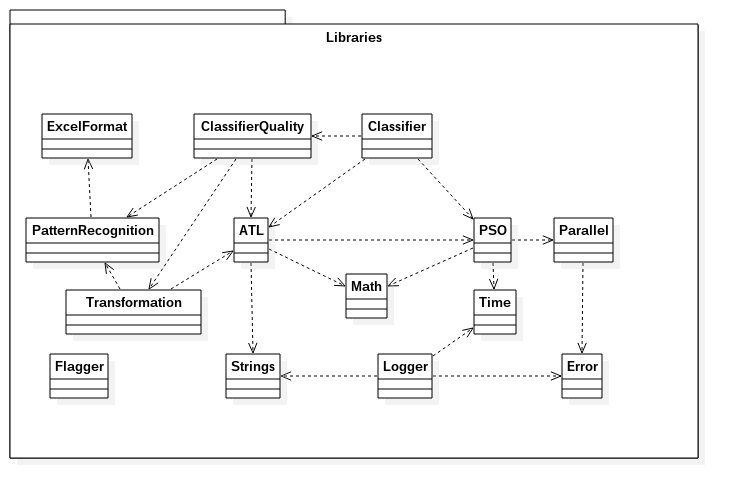
\includegraphics[width=0.9\textwidth]{../uml/dependencies.png}
    \caption{Dependencies of libraries}
    \label{fig:lib_dependencies}
\end{figure}

\newpage

%---------------------------------------------------------------
%---------------------------------------------------------------
%---------------------------------------------------------------
\subsection{PSO}

The PSO library provides interface for implementing optimizations for any problem of interest. The class overview is presented in figure~\ref{fig:lib_pso_classes}. The {\bf PSO} class is responsible for gathering all modules and running computations. {\bf FitnessUpdater, ParticleUpdater and NeighbourhoodUpdater} are pure abstracted classes providing interface for respective part of the algorithm. {\bf FitnessUpdater} calculates and updates fitness values of each particle. {\bf ParticleUpdater} is responsible for updating particle's position and velocity. Finally, {\bf NeighbourhoodUpdater} updates the neighbourhoods and finds lbest value for each particle. {\bf ParticleDecoder} is responsible for decoding the {\bf PSOObject} which is later used in {\bf FitnessUpdater} to evaluate the fitness value. In order to optimize a specific object, one must derive it from {\bf PSOObject} and the decoding method must be implemented in derived {\bf ParticleDecoder}. Finally {\bf ParticleUpdaterSpherical} and {\bf NBStarTopology} provide implementations of algorithms explained in chapter~\ref{chap:pso}.

\begin{figure}
    \centering
    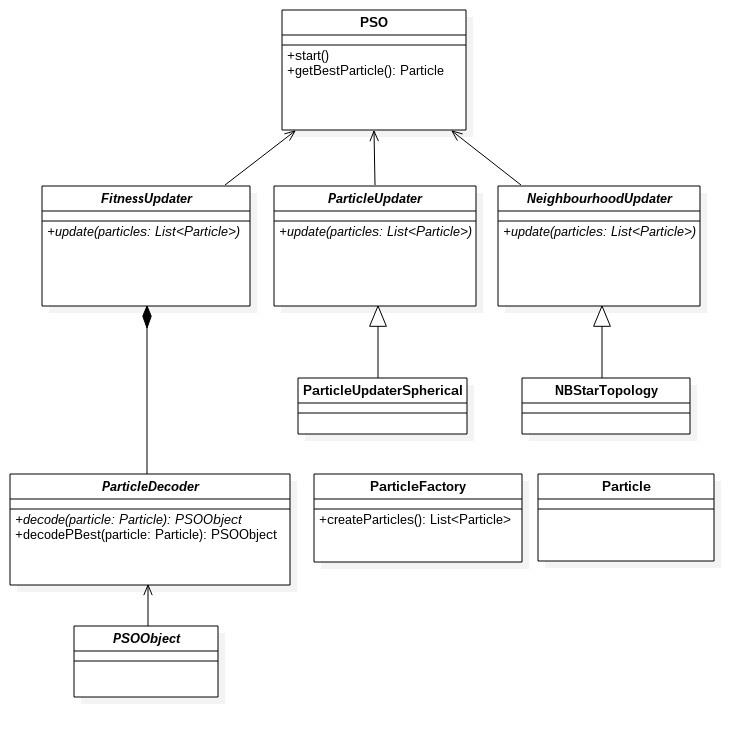
\includegraphics[width=0.7\textwidth]{../uml/pso_classes.png}
    \caption{Particle Swarm Optimization Library. Classes Association}
    \label{fig:lib_pso_classes}
\end{figure}

The PSO has been implemented using parallel CPU algorithm. The state diagram showing details of computations process is shown in figure~\ref{fig:lib_pso_states}. Since each particle can be computed independently, PSO can be easily parallelized. Each thread is assigned interval of particle indices for which it is responsible for. Simply thread synchronization between each step of the iteration is executed. The {\bf Parallel } library is used for the multi threaded functionality.

\begin{figure}
    \centering
    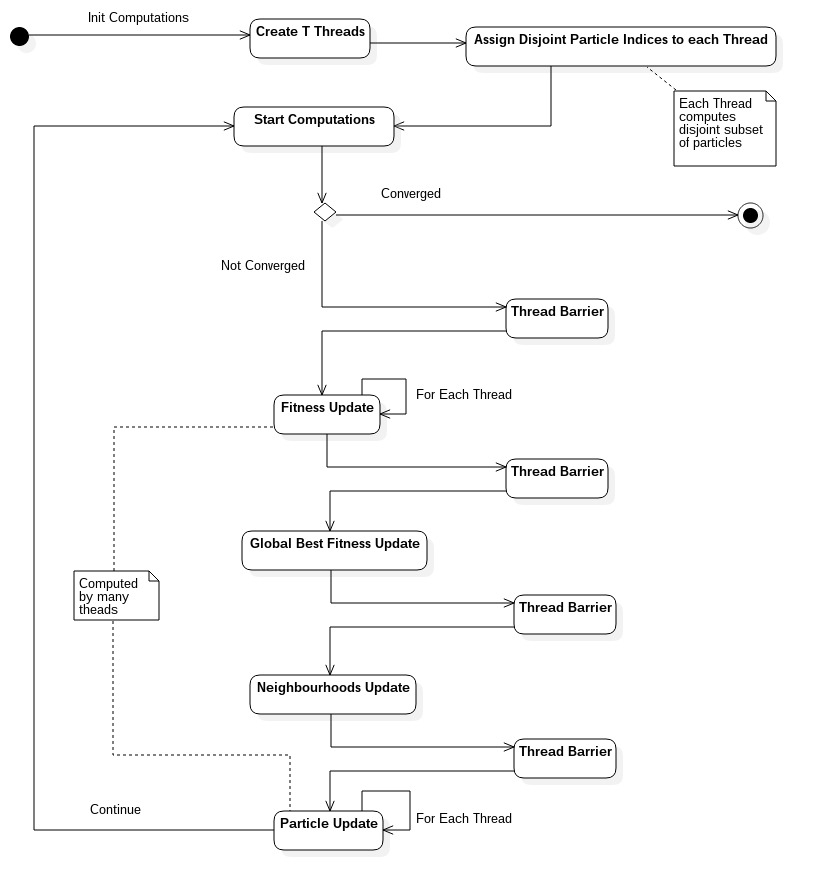
\includegraphics[width=0.9\textwidth]{../uml/pso_state.jpg}
    \caption{Particle Swarm Optimization Library. State diagram of the algorithm }
    \label{fig:lib_pso_states}
\end{figure}


%---------------------------------------------------------------
%---------------------------------------------------------------
%---------------------------------------------------------------
\subsection{ATL}

{\bf DFA} or Deterministic Finite Automaton, takes a {\bf Word} as an input and computes which {\bf State} it finishes in. {\bf TransitionFunction} allows for setting and getting transition for specific configurations. {\bf Language} class, contains also corresponding states which are used in the classification process. In that case {\bf Language} is considered to be a label and states are checked against all languages in order to classify a word to one of the languages. The classes are shown in figure~\ref{fig:lib_atl}.


\begin{figure}
    \centering
    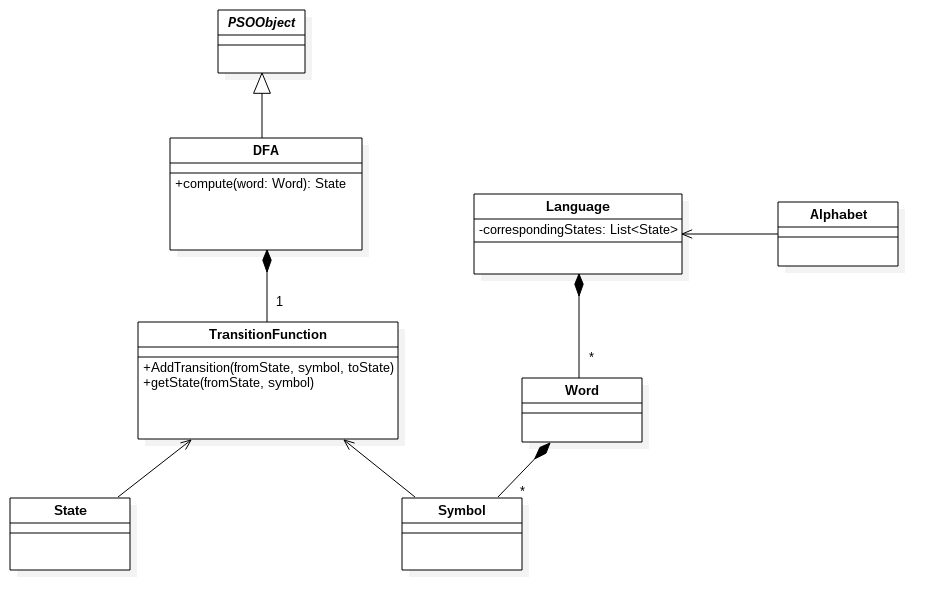
\includegraphics[width=1.0\textwidth]{../uml/atl.png}
    \caption{Automata and Languages Library. Classes Association}
    \label{fig:lib_atl}
\end{figure}


%---------------------------------------------------------------
%---------------------------------------------------------------
%---------------------------------------------------------------
\subsection{Pattern Recognition}

The classes are presented in figure~\ref{fig:lib_pt}. {\bf Class} contains a single {\bf Label} and possibly many {\bf FeatureVectors}. {\bf XLSLoader} is used to load Classes from excel files.

\begin{figure}
    \centering
    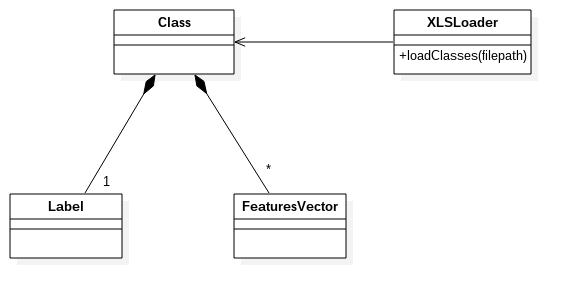
\includegraphics[width=0.7\textwidth]{../uml/pt.png}
    \caption{Pattern Recognition Library. Classes Association}
    \label{fig:lib_pt}
\end{figure}
 
%---------------------------------------------------------------
%---------------------------------------------------------------
%---------------------------------------------------------------
\subsection{Transformation}
Transformation library contains two modules: {\bf Transformation} and {\bf Transformation Analysis}. State diagram of transformation is shown in figure~\ref{fig:transform_state}. For input classes, interval of each feature must be calculated. Then the features are normalized and corresponding symbols are assigned to make up a word. All transformed words from respective class make up a language.


\begin{figure}
    \centering
    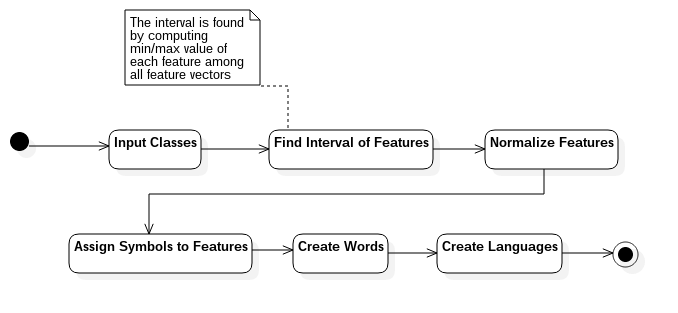
\includegraphics[width=0.8\textwidth]{../uml/transformation_state.png}
    \caption{Transformation state diagram}
    \label{fig:transform_state}
\end{figure}

The {\bf Transformation Analysis} process is illustrated in figure~\ref{fig:transform_analysis_state}. The classes are transformed to languages and similarity is computed for each pair. Then all the similarities are averaged and output as result. This process is to be repeated for different alphabet sizes.

\begin{figure}
    \centering
    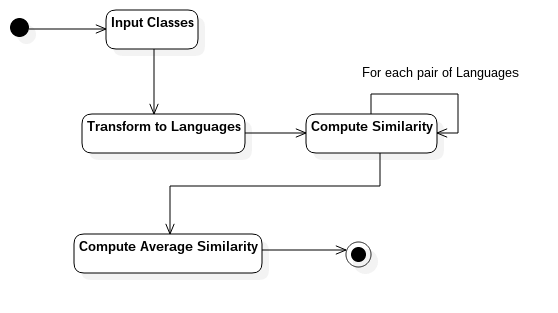
\includegraphics[width=0.8\textwidth]{../uml/transform_analysis_state.png}
    \caption{Transformation Analysis state diagram.}
    \label{fig:transform_analysis_state}
\end{figure}


%---------------------------------------------------------------
%---------------------------------------------------------------
%---------------------------------------------------------------
\subsection{Classifier}

The classes are shown in figure~\ref{fig:classifier_pso_classes}. The {\bf DFAParticleDecoder} derives from the PSO interface and implements the solution for DFA decoding. Similarly, all 8 fitness functions are implemented in derived {\bf FitnessUpdaters}. For simplicity, only two of the fitness functions are illustrated in the graph.

\begin{figure}
    \centering
    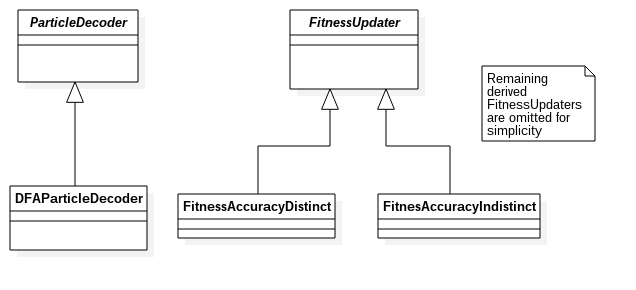
\includegraphics[width=0.8\textwidth]{../uml/classifier_pso_classes.png}
    \caption{Classifier Library.}
    \label{fig:classifier_pso_classes}
\end{figure}

%---------------------------------------------------------------
%---------------------------------------------------------------
\section{Applications}

%---------------------------------------------------------------
%---------------------------------------------------------------
%---------------------------------------------------------------
\subsection{Classifier Constructor}

The {\bf Classifier Constructor} uses all the libraries in order to conduct experiments. All of the settings can be provided by the user in a form of flags when starting the application. The application is split into two experiments: Classification based on PSO heuristics and Transformation Analysis. The Transformation Analysis experiment is an encapsulation of the {\bf Transformation} library.

The simplified process of Classification experiment is presented in figure~\ref{fig:classification_states}. The classes are loaded and transformed to languages. Languages are assigned states based on application settings and then the classifier constructor is started.

\begin{figure}
    \centering
    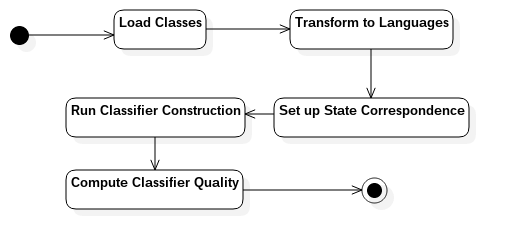
\includegraphics[width=0.6\textwidth]{../uml/classification_state.png}
    \caption{Constructing Classifier state diagram.}
    \label{fig:classification_states}
\end{figure}

\newpage

%---------------------------------------------------------------
%---------------------------------------------------------------
\section{Graphical User Interface}

%
% GUI CLASS DIAGRAM
%
\begin{wrapfigure}{c}{0.7\textwidth}
    \begin{center}
        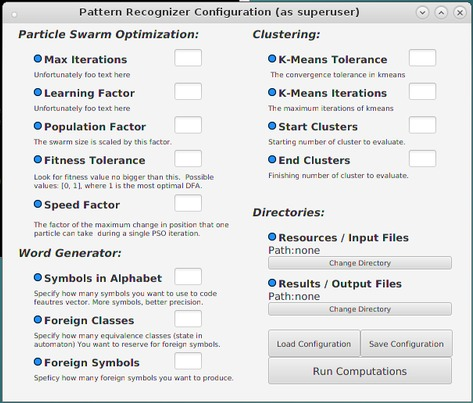
\includegraphics[width=0.7\textwidth]{images/mock_gui.jpg}
    \end{center}
    \caption{GUI Mockup}
    \label{fig:gui_look}
\end{wrapfigure}

Classes necessary to model and develop GUI are presented on figure \ref{fig:gui_classes}. On the other hand, look that we are trying to achieve is roughly sketch on figure \ref{fig:gui_look}.

As one could image, because of simplicity of the interface, there is nothing fancy in class diagram. \texttt{MainWindow} handles loading .fxml file and starting the application. On the oder hand, class \texttt{MainWindowControls} is in charge of events processing. It handles any event occurred regarding user interface objects and performs appropriate actions. Since main functionality of this part of the application is to set up global configurations, when some value within an user interface object will change, so will corresponding entry in configuration file. One can easily load and save configurations files, as well as changing directory of input and output files. Presented figure \ref{fig:gui_look}, depicting design of the application, is definitely not the final one and in future it might contain e.g. text labels with more informations about features or some loading bars. Main look of the program should be defined in .fxml, which will not be presented in this paper due to its irrelevancy and numerous way of implementations. 

\begin{figure}[H]
    \centering
    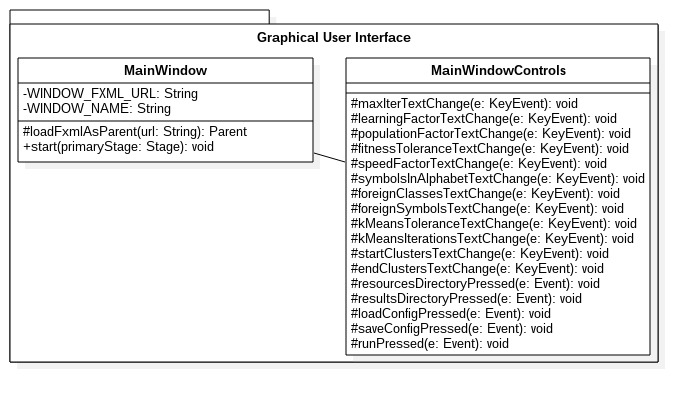
\includegraphics[width=0.9\textwidth]{images/gui.jpg}
    \caption{Class diagram of gui classes}
    \label{fig:gui_classes}
\end{figure}



%---------------------------------------------------------------
\begin{thebibliography}{1}
    
    \bibitem{pso_origin} 
    Eberhart, R. C. and Kennedy, J. A new optimizer using particle swarm theory. Proceedings of the sixth international symposium on micro machine and human science pp. 39-43. IEEE service center, Piscataway, NJ, Nagoya, Japan, 1995.
    
    \bibitem{pso_anal}
    Maurice Clerc. Stagnation analysis in particle swarm optimization or what happens when nothing happens, http://hal.archives-ouvertes.fr/hal-00122031. Technical report, 2006.

    \bibitem{pso_bias} 
    William M. Spears, Derek T. Green and Diana F. Spears. Biases in particle swarm optimization. International Journal of Swarm Intelligence Research, 1(2):34-57, 2010.

    \bibitem{pso_11}
    M. Clerc. (2011). Standard Particle Swarm Optimisation Available: http://hal.archives-ouvertes.fr/hal-00764996 
    
    \bibitem{bishop_book} Christopher M. Bishop; Pattern Recognition and Machine Learning (Information Science and Statistics)
    
	\bibitem{Homenda_2014} Homenda W., Luckner M., Pedrycz W., Classification with rejection based on various SVM techniques, Proceedings of the WCCI 2014 IEEE World Congress on Computational Intelligence, pp. 3480-3487, Beijing, China, 2014     
    
	\bibitem{semi_supervised} Xiaojin Zhu and Andrew B.Goldberg, Synthesis Lectures on Artificial Intelligence and Machine Learning, 2009, Vol. 3, No. 1 , Pages 1-130    
	
    \bibitem{semi_supervised2} Xiaojin Zhu, Semi-Supervised Learning Literature Survey, 2006

	
	\bibitem{images_learning_types} Anuj R. Shah1, Christopher S. Oehmen, Bobbie-Jo Webb-Robertson, SVM-Hustle - An iterative semi-supervised machine learning approach for pairwise protein remote homology detection 
    
	\bibitem{duch_uuu} Robert P.W. Duin, Elzbieta Pekalska, The Science of Pattern Recognition. Achievements and Perspectives, Studies in Computational Intelligence, chapter Challenges for Computational Intelligence, page 63 , 2007
    
    \bibitem{excel_format} http://www.codeproject.com/Articles/42504/ExcelFormat-Library
	
    \bibitem{hc_1} H.-G. Beyer, “Toward a Theory of Evolution Strategies: The (mu, lambda)-Theory,” Evolutionary Computation, vol. 2, no. 4, pp. 381-407, 1994.
    
    \bibitem{hc_2} M. Mitchell, J. Holland, and S. Forrest, “When Will a Genetic Algorithm Outperform Hill Climbing?” Advances in Neural Information Processing Systems 6, J. Cowan, G. Tesauro, and J. Alspector,
    eds., pp. 51-58, San Mateo, Calif.: Morgan Kaufman, 1994.
    
    \bibitem{hc_3} Russel, S. J., Norvig, P. (2003). Artificial intelligence: a modern approach. Upper Saddle River, N.J., Prentice Hall/Pearson Education.
    
    \bibitem{digits_db}LeCun, Y., Cortes, C., Burges, C.: The MNIST database of handwritten digits (1996). http://yann.lecun.com/exdb/mnist/
    
    \bibitem{hc_4}S.M. Lucas and T.J. Reynolds, “Learning DFA: Evolution versus Evidence Driven State Merging,” Proc. Congress Evolutionary Computation, pp. 351-358, 2003.
    
    \bibitem{handwritten_digits_intro} Subset of the MNIST Database, found on http://sujitpal.blogspot.com/2014/07/handwritten-digit-recognition-with.html

\end{thebibliography}



\newpage
\chapter*{Footer}
{\bf Legal:} The vectors of features used in this thesis are given by the supervisor and cannot be used without written permission for any aim other than this thesis.
\newpage


\makestatement
\end{document}
